\documentclass[twocolumn,20pt,fleqn]{extarticle}
\usepackage{color}
\usepackage{geometry}
\usepackage[normalem]{ulem}
\usepackage{cancel}
\usepackage{dingbat}
\usepackage{marginnote}
\usepackage{amsmath}
\usepackage{amsthm}
\usepackage{amssymb}
\usepackage{amsfonts}
\usepackage{mathtools}
\usepackage{tcolorbox}
\usepackage{multicol}
\usepackage{tikz}
\usepackage{tikz-cd}
\usepackage{wrapfig}
\usepackage{caption}
%\usepackage{draftwatermark}

\usetikzlibrary{calc}

\setlength{\parindent}{0pt}
\setlength{\parskip}{0.5em}
\makeatletter
\renewcommand{\@seccntformat}[1]{}
\makeatother

\geometry{paperwidth=34cm, paperheight=19cm, margin=0.5cm}

\newcommand{\clr}[2]{{\color{#1} #2}}
\newcommand{\alert}[1]{{\color{red} #1}}
\newcommand{\ovrbrc}[2]{\overbrace{#2}^{#1}}
\newcommand{\undrbrc}[2]{\underbrace{#2}_{#1}}
\newcommand{\lnspc}{\vspace{1cm}}
\newcommand{\sep}{\vspace{0.5cm}}
\newcommand{\e}{\textrm{e}}
%\newcommand{\dydx}[2]{\frac{\mathrm{d}}}

\theoremstyle{plain}
\newtheorem*{theorem}{Theorem}
\newtheorem*{proposition}{Proposition}
\newtheorem*{lemma}{Lemma}
\newtheorem*{corollary}{Corollary}

\theoremstyle{definition}
\newtheorem*{exercise}{Exercise}
\newtheorem*{definition}{Definition}
\newtheorem*{example}{Example}
\newtheorem*{exmpls}{Examples}


\theoremstyle{remark}
\newtheorem*{remark}{Remark}
\newtheorem*{note}{Note}

\newenvironment*{examples}{\begin{exmpls} ~ \begin{enumerate}}{\end{enumerate}\end{exmpls}}

\begin{document}



\clearpage


\subsection{Notation: Sets}


\clearpage


\subsection{Notation: Sets}


\begin{tikzpicture}
\draw[thin,->] (-5,0) -- (5,0) node[anchor=west] {$x$};
\end{tikzpicture}


\clearpage


\subsection{Notation: Sets}


\begin{tikzpicture}
\draw[thin,->] (-5,0) -- (5,0) node[anchor=west] {$x$};
\foreach \x in {-4,-3,-2,-1,0,1,2,3,4}
\draw (\x cm,2pt) -- (\x cm,-2pt);
\end{tikzpicture}


\clearpage


\subsection{Notation: Sets}


\begin{tikzpicture}
\draw[thin,->] (-5,0) -- (5,0) node[anchor=west] {$x$};
\foreach \x in {-4,-3,-2,-1,0,1,2,3,4}
\draw (\x cm,2pt) -- (\x cm,-2pt);
\foreach \x in {-4,-3,-2,-1,0,1,2,3,4}
\node[anchor=north] at (\x cm,0) {\footnotesize \x};
\end{tikzpicture}


\clearpage


\subsection{Notation: Sets}


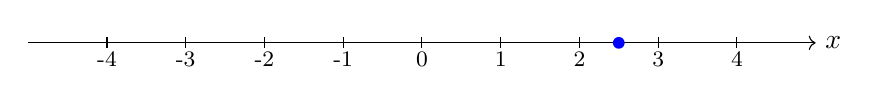
\begin{tikzpicture}
\draw[thin,->] (-5,0) -- (5,0) node[anchor=west] {$x$};
\foreach \x in {-4,-3,-2,-1,0,1,2,3,4}
\draw (\x cm,2pt) -- (\x cm,-2pt);
\foreach \x in {-4,-3,-2,-1,0,1,2,3,4}
\node[anchor=north] at (\x cm,0) {\footnotesize \x};
\node at (2.5 cm,0)[circle,fill,inner sep=1.5pt,color=blue] {};
\end{tikzpicture}



\begin{tikzpicture}
\draw[thin,->] (-5,0) -- (5,0) node[anchor=west] {$x$};
\foreach \x in {-4,-3,-2,-1,0,1,2,3,4}
\draw (\x cm,2pt) -- (\x cm,-2pt);
\end{tikzpicture}


\clearpage


\subsection{Notation: Sets}


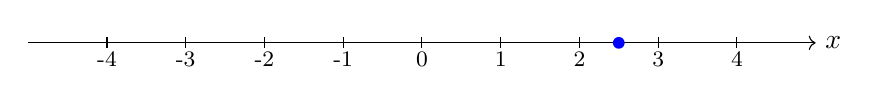
\begin{tikzpicture}
\draw[thin,->] (-5,0) -- (5,0) node[anchor=west] {$x$};
\foreach \x in {-4,-3,-2,-1,0,1,2,3,4}
\draw (\x cm,2pt) -- (\x cm,-2pt);
\foreach \x in {-4,-3,-2,-1,0,1,2,3,4}
\node[anchor=north] at (\x cm,0) {\footnotesize \x};
\node at (2.5 cm,0)[circle,fill,inner sep=1.5pt,color=blue] {};
\end{tikzpicture}



\begin{tikzpicture}
\draw[thin,->] (-5,0) -- (5,0) node[anchor=west] {$x$};
\foreach \x in {-4,-3,-2,-1,0,1,2,3,4}
\draw (\x cm,2pt) -- (\x cm,-2pt);
\foreach \x in {-4,-3,-2,-1,1,2,3,4}
\node[anchor=north] at (\x cm,0) {\footnotesize \x};
\draw[thin,->] (0,-5) -- (0,5) node[anchor=south] {$y$};
\foreach \y in {-4,-3,-2,-1,0,1,2,3,4}
\draw (2pt, \y cm) -- (-2pt, \y cm);
\end{tikzpicture}


\clearpage


\subsection{Notation: Sets}


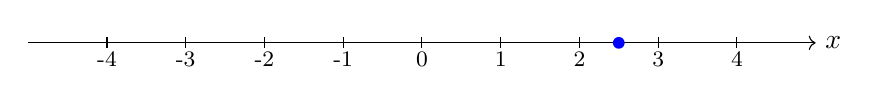
\begin{tikzpicture}
\draw[thin,->] (-5,0) -- (5,0) node[anchor=west] {$x$};
\foreach \x in {-4,-3,-2,-1,0,1,2,3,4}
\draw (\x cm,2pt) -- (\x cm,-2pt);
\foreach \x in {-4,-3,-2,-1,0,1,2,3,4}
\node[anchor=north] at (\x cm,0) {\footnotesize \x};
\node at (2.5 cm,0)[circle,fill,inner sep=1.5pt,color=blue] {};
\end{tikzpicture}



\begin{tikzpicture}
\draw[thin,->] (-5,0) -- (5,0) node[anchor=west] {$x$};
\foreach \x in {-4,-3,-2,-1,0,1,2,3,4}
\draw (\x cm,2pt) -- (\x cm,-2pt);
\foreach \x in {-4,-3,-2,-1,1,2,3,4}
\node[anchor=north] at (\x cm,0) {\footnotesize \x};
\draw[thin,->] (0,-5) -- (0,5) node[anchor=south] {$y$};
\foreach \y in {-4,-3,-2,-1,0,1,2,3,4}
\draw (2pt, \y cm) -- (-2pt, \y cm);
\foreach \y in {-4,-3,-2,-1,1,2,3,4}
\node[anchor=west] at (0, \y cm) {\footnotesize \y};
\end{tikzpicture}


\clearpage


\subsection{Notation: Sets}


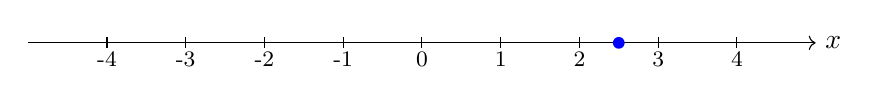
\begin{tikzpicture}
\draw[thin,->] (-5,0) -- (5,0) node[anchor=west] {$x$};
\foreach \x in {-4,-3,-2,-1,0,1,2,3,4}
\draw (\x cm,2pt) -- (\x cm,-2pt);
\foreach \x in {-4,-3,-2,-1,0,1,2,3,4}
\node[anchor=north] at (\x cm,0) {\footnotesize \x};
\node at (2.5 cm,0)[circle,fill,inner sep=1.5pt,color=blue] {};
\end{tikzpicture}



\begin{tikzpicture}
\draw[thin,->] (-5,0) -- (5,0) node[anchor=west] {$x$};
\foreach \x in {-4,-3,-2,-1,0,1,2,3,4}
\draw (\x cm,2pt) -- (\x cm,-2pt);
\foreach \x in {-4,-3,-2,-1,1,2,3,4}
\node[anchor=north] at (\x cm,0) {\footnotesize \x};
\draw[thin,->] (0,-5) -- (0,5) node[anchor=south] {$y$};
\foreach \y in {-4,-3,-2,-1,0,1,2,3,4}
\draw (2pt, \y cm) -- (-2pt, \y cm);
\foreach \y in {-4,-3,-2,-1,1,2,3,4}
\node[anchor=west] at (0, \y cm) {\footnotesize \y};
\node[anchor=north west] at (0,0) {\footnotesize O};
;
\end{tikzpicture}
 


\newpage


\sep






\clearpage


\subsection{Notation: Sets}


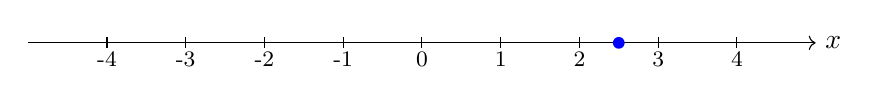
\begin{tikzpicture}
\draw[thin,->] (-5,0) -- (5,0) node[anchor=west] {$x$};
\foreach \x in {-4,-3,-2,-1,0,1,2,3,4}
\draw (\x cm,2pt) -- (\x cm,-2pt);
\foreach \x in {-4,-3,-2,-1,0,1,2,3,4}
\node[anchor=north] at (\x cm,0) {\footnotesize \x};
\node at (2.5 cm,0)[circle,fill,inner sep=1.5pt,color=blue] {};
\end{tikzpicture}



\begin{tikzpicture}
\draw[thin,->] (-5,0) -- (5,0) node[anchor=west] {$x$};
\foreach \x in {-4,-3,-2,-1,0,1,2,3,4}
\draw (\x cm,2pt) -- (\x cm,-2pt);
\foreach \x in {-4,-3,-2,-1,1,2,3,4}
\node[anchor=north] at (\x cm,0) {\footnotesize \x};
\draw[thin,->] (0,-5) -- (0,5) node[anchor=south] {$y$};
\foreach \y in {-4,-3,-2,-1,0,1,2,3,4}
\draw (2pt, \y cm) -- (-2pt, \y cm);
\foreach \y in {-4,-3,-2,-1,1,2,3,4}
\node[anchor=west] at (0, \y cm) {\footnotesize \y};
\node[anchor=north west] at (0,0) {\footnotesize O};
\node at (1,1)[circle,fill,inner sep=1.5pt,color=blue]{} ;
\end{tikzpicture}
 


\newpage

 Point: $(1,1)$
\sep






\clearpage


\subsection{Notation: Sets}


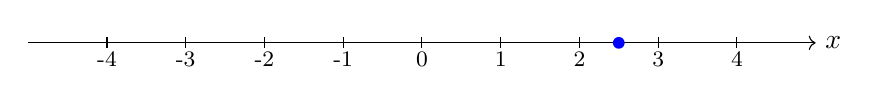
\begin{tikzpicture}
\draw[thin,->] (-5,0) -- (5,0) node[anchor=west] {$x$};
\foreach \x in {-4,-3,-2,-1,0,1,2,3,4}
\draw (\x cm,2pt) -- (\x cm,-2pt);
\foreach \x in {-4,-3,-2,-1,0,1,2,3,4}
\node[anchor=north] at (\x cm,0) {\footnotesize \x};
\node at (2.5 cm,0)[circle,fill,inner sep=1.5pt,color=blue] {};
\end{tikzpicture}



\begin{tikzpicture}
\draw[thin,->] (-5,0) -- (5,0) node[anchor=west] {$x$};
\foreach \x in {-4,-3,-2,-1,0,1,2,3,4}
\draw (\x cm,2pt) -- (\x cm,-2pt);
\foreach \x in {-4,-3,-2,-1,1,2,3,4}
\node[anchor=north] at (\x cm,0) {\footnotesize \x};
\draw[thin,->] (0,-5) -- (0,5) node[anchor=south] {$y$};
\foreach \y in {-4,-3,-2,-1,0,1,2,3,4}
\draw (2pt, \y cm) -- (-2pt, \y cm);
\foreach \y in {-4,-3,-2,-1,1,2,3,4}
\node[anchor=west] at (0, \y cm) {\footnotesize \y};
\node[anchor=north west] at (0,0) {\footnotesize O};
\node at (1,1)[circle,fill,inner sep=1.5pt,color=blue]{} ;
\end{tikzpicture}
 


\newpage

 Point: $(1,1)\in \mathbb{R}^2$ 
\sep







\clearpage


\subsection{Notation: Sets}


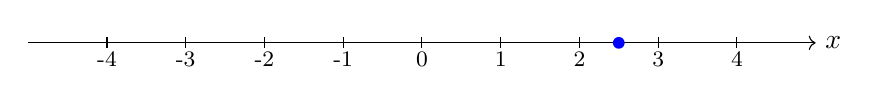
\begin{tikzpicture}
\draw[thin,->] (-5,0) -- (5,0) node[anchor=west] {$x$};
\foreach \x in {-4,-3,-2,-1,0,1,2,3,4}
\draw (\x cm,2pt) -- (\x cm,-2pt);
\foreach \x in {-4,-3,-2,-1,0,1,2,3,4}
\node[anchor=north] at (\x cm,0) {\footnotesize \x};
\node at (2.5 cm,0)[circle,fill,inner sep=1.5pt,color=blue] {};
\end{tikzpicture}



\begin{tikzpicture}
\draw[thin,->] (-5,0) -- (5,0) node[anchor=west] {$x$};
\foreach \x in {-4,-3,-2,-1,0,1,2,3,4}
\draw (\x cm,2pt) -- (\x cm,-2pt);
\foreach \x in {-4,-3,-2,-1,1,2,3,4}
\node[anchor=north] at (\x cm,0) {\footnotesize \x};
\draw[thin,->] (0,-5) -- (0,5) node[anchor=south] {$y$};
\foreach \y in {-4,-3,-2,-1,0,1,2,3,4}
\draw (2pt, \y cm) -- (-2pt, \y cm);
\foreach \y in {-4,-3,-2,-1,1,2,3,4}
\node[anchor=west] at (0, \y cm) {\footnotesize \y};
\node[anchor=north west] at (0,0) {\footnotesize O};
\node at  (1,2) [circle,fill,inner sep=1.5pt,color=blue]{} ;
\end{tikzpicture}
 


\newpage

 Point: $ (1,2) \in \mathbb{R}^2$ 
\sep








\clearpage


\subsection{Notation: Sets}


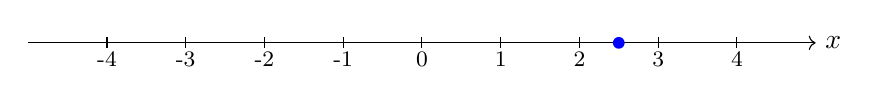
\begin{tikzpicture}
\draw[thin,->] (-5,0) -- (5,0) node[anchor=west] {$x$};
\foreach \x in {-4,-3,-2,-1,0,1,2,3,4}
\draw (\x cm,2pt) -- (\x cm,-2pt);
\foreach \x in {-4,-3,-2,-1,0,1,2,3,4}
\node[anchor=north] at (\x cm,0) {\footnotesize \x};
\node at (2.5 cm,0)[circle,fill,inner sep=1.5pt,color=blue] {};
\end{tikzpicture}



\begin{tikzpicture}
\draw[thin,->] (-5,0) -- (5,0) node[anchor=west] {$x$};
\foreach \x in {-4,-3,-2,-1,0,1,2,3,4}
\draw (\x cm,2pt) -- (\x cm,-2pt);
\foreach \x in {-4,-3,-2,-1,1,2,3,4}
\node[anchor=north] at (\x cm,0) {\footnotesize \x};
\draw[thin,->] (0,-5) -- (0,5) node[anchor=south] {$y$};
\foreach \y in {-4,-3,-2,-1,0,1,2,3,4}
\draw (2pt, \y cm) -- (-2pt, \y cm);
\foreach \y in {-4,-3,-2,-1,1,2,3,4}
\node[anchor=west] at (0, \y cm) {\footnotesize \y};
\node[anchor=north west] at (0,0) {\footnotesize O};
\node at  (1,2.5) [circle,fill,inner sep=1.5pt,color=blue]{} ;
\end{tikzpicture}
 


\newpage

 Point: $ (1,2.5) \in \mathbb{R}^2$ 
\sep









\clearpage


\subsection{Notation: Sets}


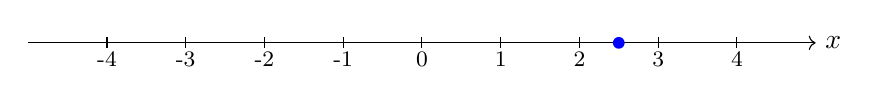
\begin{tikzpicture}
\draw[thin,->] (-5,0) -- (5,0) node[anchor=west] {$x$};
\foreach \x in {-4,-3,-2,-1,0,1,2,3,4}
\draw (\x cm,2pt) -- (\x cm,-2pt);
\foreach \x in {-4,-3,-2,-1,0,1,2,3,4}
\node[anchor=north] at (\x cm,0) {\footnotesize \x};
\node at (2.5 cm,0)[circle,fill,inner sep=1.5pt,color=blue] {};
\end{tikzpicture}



\begin{tikzpicture}
\draw[thin,->] (-5,0) -- (5,0) node[anchor=west] {$x$};
\foreach \x in {-4,-3,-2,-1,0,1,2,3,4}
\draw (\x cm,2pt) -- (\x cm,-2pt);
\foreach \x in {-4,-3,-2,-1,1,2,3,4}
\node[anchor=north] at (\x cm,0) {\footnotesize \x};
\draw[thin,->] (0,-5) -- (0,5) node[anchor=south] {$y$};
\foreach \y in {-4,-3,-2,-1,0,1,2,3,4}
\draw (2pt, \y cm) -- (-2pt, \y cm);
\foreach \y in {-4,-3,-2,-1,1,2,3,4}
\node[anchor=west] at (0, \y cm) {\footnotesize \y};
\node[anchor=north west] at (0,0) {\footnotesize O};
\node at  (3,2) [circle,fill,inner sep=1.5pt,color=blue]{} ;
\end{tikzpicture}
 


\newpage

 Point: $ (3,2) \in \mathbb{R}^2$ 
\sep










\clearpage


\subsection{Notation: Sets}


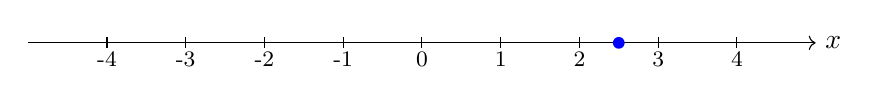
\begin{tikzpicture}
\draw[thin,->] (-5,0) -- (5,0) node[anchor=west] {$x$};
\foreach \x in {-4,-3,-2,-1,0,1,2,3,4}
\draw (\x cm,2pt) -- (\x cm,-2pt);
\foreach \x in {-4,-3,-2,-1,0,1,2,3,4}
\node[anchor=north] at (\x cm,0) {\footnotesize \x};
\node at (2.5 cm,0)[circle,fill,inner sep=1.5pt,color=blue] {};
\end{tikzpicture}



\begin{tikzpicture}
\draw[thin,->] (-5,0) -- (5,0) node[anchor=west] {$x$};
\foreach \x in {-4,-3,-2,-1,0,1,2,3,4}
\draw (\x cm,2pt) -- (\x cm,-2pt);
\foreach \x in {-4,-3,-2,-1,1,2,3,4}
\node[anchor=north] at (\x cm,0) {\footnotesize \x};
\draw[thin,->] (0,-5) -- (0,5) node[anchor=south] {$y$};
\foreach \y in {-4,-3,-2,-1,0,1,2,3,4}
\draw (2pt, \y cm) -- (-2pt, \y cm);
\foreach \y in {-4,-3,-2,-1,1,2,3,4}
\node[anchor=west] at (0, \y cm) {\footnotesize \y};
\node[anchor=north west] at (0,0) {\footnotesize O};
\node at (3,2)[circle,fill,inner sep=1.5pt,color=blue]{} ;
\end{tikzpicture}
 


\newpage

  
\sep












\clearpage


\subsection{Notation: Sets}


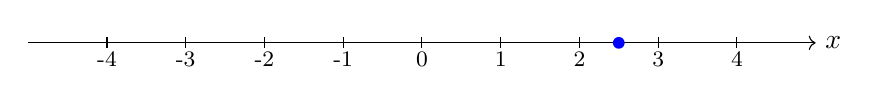
\begin{tikzpicture}
\draw[thin,->] (-5,0) -- (5,0) node[anchor=west] {$x$};
\foreach \x in {-4,-3,-2,-1,0,1,2,3,4}
\draw (\x cm,2pt) -- (\x cm,-2pt);
\foreach \x in {-4,-3,-2,-1,0,1,2,3,4}
\node[anchor=north] at (\x cm,0) {\footnotesize \x};
\node at (2.5 cm,0)[circle,fill,inner sep=1.5pt,color=blue] {};
\end{tikzpicture}



\begin{tikzpicture}
\draw[thin,->] (-5,0) -- (5,0) node[anchor=west] {$x$};
\foreach \x in {-4,-3,-2,-1,0,1,2,3,4}
\draw (\x cm,2pt) -- (\x cm,-2pt);
\foreach \x in {-4,-3,-2,-1,1,2,3,4}
\node[anchor=north] at (\x cm,0) {\footnotesize \x};
\draw[thin,->] (0,-5) -- (0,5) node[anchor=south] {$y$};
\foreach \y in {-4,-3,-2,-1,0,1,2,3,4}
\draw (2pt, \y cm) -- (-2pt, \y cm);
\foreach \y in {-4,-3,-2,-1,1,2,3,4}
\node[anchor=west] at (0, \y cm) {\footnotesize \y};
\node[anchor=north west] at (0,0) {\footnotesize O};
\node at (3,2)[circle,fill,inner sep=1.5pt,color=blue]{} ; \node at (1,2)[circle,fill,inner sep=1.5pt,color=blue]{} ;
\end{tikzpicture}
 


\newpage

  
\sep












\clearpage


\subsection{Notation: Sets}


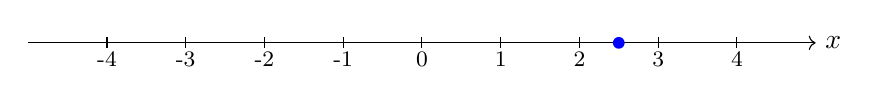
\begin{tikzpicture}
\draw[thin,->] (-5,0) -- (5,0) node[anchor=west] {$x$};
\foreach \x in {-4,-3,-2,-1,0,1,2,3,4}
\draw (\x cm,2pt) -- (\x cm,-2pt);
\foreach \x in {-4,-3,-2,-1,0,1,2,3,4}
\node[anchor=north] at (\x cm,0) {\footnotesize \x};
\node at (2.5 cm,0)[circle,fill,inner sep=1.5pt,color=blue] {};
\end{tikzpicture}



\begin{tikzpicture}
\draw[thin,->] (-5,0) -- (5,0) node[anchor=west] {$x$};
\foreach \x in {-4,-3,-2,-1,0,1,2,3,4}
\draw (\x cm,2pt) -- (\x cm,-2pt);
\foreach \x in {-4,-3,-2,-1,1,2,3,4}
\node[anchor=north] at (\x cm,0) {\footnotesize \x};
\draw[thin,->] (0,-5) -- (0,5) node[anchor=south] {$y$};
\foreach \y in {-4,-3,-2,-1,0,1,2,3,4}
\draw (2pt, \y cm) -- (-2pt, \y cm);
\foreach \y in {-4,-3,-2,-1,1,2,3,4}
\node[anchor=west] at (0, \y cm) {\footnotesize \y};
\node[anchor=north west] at (0,0) {\footnotesize O};
\node at (3,2)[circle,fill,inner sep=1.5pt,color=blue]{} ; \node at (1,2)[circle,fill,inner sep=1.5pt,color=blue]{} ;\
\node at (1,1)[circle,fill,inner sep=1.5pt,color=blue]{} ;
\end{tikzpicture}
 


\newpage

  
\sep













\clearpage


\subsection{Notation: Sets}


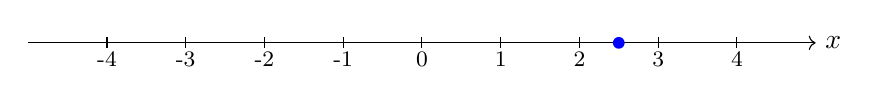
\begin{tikzpicture}
\draw[thin,->] (-5,0) -- (5,0) node[anchor=west] {$x$};
\foreach \x in {-4,-3,-2,-1,0,1,2,3,4}
\draw (\x cm,2pt) -- (\x cm,-2pt);
\foreach \x in {-4,-3,-2,-1,0,1,2,3,4}
\node[anchor=north] at (\x cm,0) {\footnotesize \x};
\node at (2.5 cm,0)[circle,fill,inner sep=1.5pt,color=blue] {};
\end{tikzpicture}



\begin{tikzpicture}
\draw[thin,->] (-5,0) -- (5,0) node[anchor=west] {$x$};
\foreach \x in {-4,-3,-2,-1,0,1,2,3,4}
\draw (\x cm,2pt) -- (\x cm,-2pt);
\foreach \x in {-4,-3,-2,-1,1,2,3,4}
\node[anchor=north] at (\x cm,0) {\footnotesize \x};
\draw[thin,->] (0,-5) -- (0,5) node[anchor=south] {$y$};
\foreach \y in {-4,-3,-2,-1,0,1,2,3,4}
\draw (2pt, \y cm) -- (-2pt, \y cm);
\foreach \y in {-4,-3,-2,-1,1,2,3,4}
\node[anchor=west] at (0, \y cm) {\footnotesize \y};
\node[anchor=north west] at (0,0) {\footnotesize O};
\node at (3,2)[circle,fill,inner sep=1.5pt,color=blue]{} ; \node at (1,2)[circle,fill,inner sep=1.5pt,color=blue]{} ;\
\node at (1,1)[circle,fill,inner sep=1.5pt,color=blue]{} ;
\end{tikzpicture}
 


\newpage

 $\{(1,1), (1,2), (1,3)\} $  
\sep














\clearpage


\subsection{Notation: Sets}


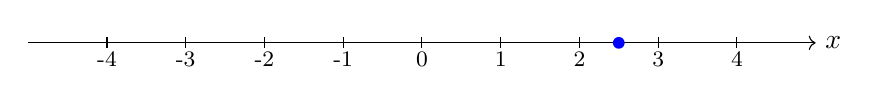
\begin{tikzpicture}
\draw[thin,->] (-5,0) -- (5,0) node[anchor=west] {$x$};
\foreach \x in {-4,-3,-2,-1,0,1,2,3,4}
\draw (\x cm,2pt) -- (\x cm,-2pt);
\foreach \x in {-4,-3,-2,-1,0,1,2,3,4}
\node[anchor=north] at (\x cm,0) {\footnotesize \x};
\node at (2.5 cm,0)[circle,fill,inner sep=1.5pt,color=blue] {};
\end{tikzpicture}



\begin{tikzpicture}
\draw[thin,->] (-5,0) -- (5,0) node[anchor=west] {$x$};
\foreach \x in {-4,-3,-2,-1,0,1,2,3,4}
\draw (\x cm,2pt) -- (\x cm,-2pt);
\foreach \x in {-4,-3,-2,-1,1,2,3,4}
\node[anchor=north] at (\x cm,0) {\footnotesize \x};
\draw[thin,->] (0,-5) -- (0,5) node[anchor=south] {$y$};
\foreach \y in {-4,-3,-2,-1,0,1,2,3,4}
\draw (2pt, \y cm) -- (-2pt, \y cm);
\foreach \y in {-4,-3,-2,-1,1,2,3,4}
\node[anchor=west] at (0, \y cm) {\footnotesize \y};
\node[anchor=north west] at (0,0) {\footnotesize O};
\node at (3,2)[circle,fill,inner sep=1.5pt,color=blue]{} ; \node at (1,2)[circle,fill,inner sep=1.5pt,color=blue]{} ;\
\node at (1,1)[circle,fill,inner sep=1.5pt,color=blue]{} ;
\end{tikzpicture}
 


\newpage

 $ S:= \{(1,1), (1,2), (1,3)\} $  
\sep















\clearpage


\subsection{Notation: Sets}


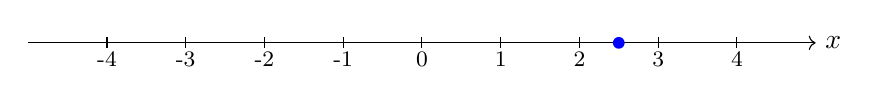
\begin{tikzpicture}
\draw[thin,->] (-5,0) -- (5,0) node[anchor=west] {$x$};
\foreach \x in {-4,-3,-2,-1,0,1,2,3,4}
\draw (\x cm,2pt) -- (\x cm,-2pt);
\foreach \x in {-4,-3,-2,-1,0,1,2,3,4}
\node[anchor=north] at (\x cm,0) {\footnotesize \x};
\node at (2.5 cm,0)[circle,fill,inner sep=1.5pt,color=blue] {};
\end{tikzpicture}



\begin{tikzpicture}
\draw[thin,->] (-5,0) -- (5,0) node[anchor=west] {$x$};
\foreach \x in {-4,-3,-2,-1,0,1,2,3,4}
\draw (\x cm,2pt) -- (\x cm,-2pt);
\foreach \x in {-4,-3,-2,-1,1,2,3,4}
\node[anchor=north] at (\x cm,0) {\footnotesize \x};
\draw[thin,->] (0,-5) -- (0,5) node[anchor=south] {$y$};
\foreach \y in {-4,-3,-2,-1,0,1,2,3,4}
\draw (2pt, \y cm) -- (-2pt, \y cm);
\foreach \y in {-4,-3,-2,-1,1,2,3,4}
\node[anchor=west] at (0, \y cm) {\footnotesize \y};
\node[anchor=north west] at (0,0) {\footnotesize O};
\node at (3,2)[circle,fill,inner sep=1.5pt,color=blue]{} ; \node at (1,2)[circle,fill,inner sep=1.5pt,color=blue]{} ;\
\node at (1,1)[circle,fill,inner sep=1.5pt,color=blue]{} ;
\end{tikzpicture}
 


\newpage

 $ S:= \{(1,1), (1,2), (1,3)\}  \subset \mathbb{R}^2 $  
\sep





















\clearpage


\subsection{Notation: Sets}


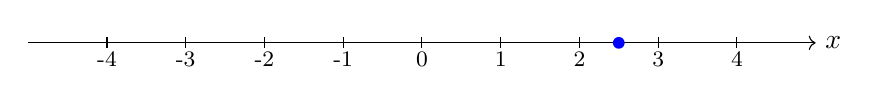
\begin{tikzpicture}
\draw[thin,->] (-5,0) -- (5,0) node[anchor=west] {$x$};
\foreach \x in {-4,-3,-2,-1,0,1,2,3,4}
\draw (\x cm,2pt) -- (\x cm,-2pt);
\foreach \x in {-4,-3,-2,-1,0,1,2,3,4}
\node[anchor=north] at (\x cm,0) {\footnotesize \x};
\node at (2.5 cm,0)[circle,fill,inner sep=1.5pt,color=blue] {};
\end{tikzpicture}



\begin{tikzpicture}
\draw[thin,->] (-5,0) -- (5,0) node[anchor=west] {$x$};
\foreach \x in {-4,-3,-2,-1,0,1,2,3,4}
\draw (\x cm,2pt) -- (\x cm,-2pt);
\foreach \x in {-4,-3,-2,-1,1,2,3,4}
\node[anchor=north] at (\x cm,0) {\footnotesize \x};
\draw[thin,->] (0,-5) -- (0,5) node[anchor=south] {$y$};
\foreach \y in {-4,-3,-2,-1,0,1,2,3,4}
\draw (2pt, \y cm) -- (-2pt, \y cm);
\foreach \y in {-4,-3,-2,-1,1,2,3,4}
\node[anchor=west] at (0, \y cm) {\footnotesize \y};
\node[anchor=north west] at (0,0) {\footnotesize O};
 \draw[thin,color=blue] (-3,-5) -- (5,4); ;
\end{tikzpicture}
 


\newpage

 $ S:= \{(1,1), (1,2), (1,3)\}  \subset \mathbb{R}^2 $  
\sep


















A line,



\clearpage


\subsection{Notation: Sets}


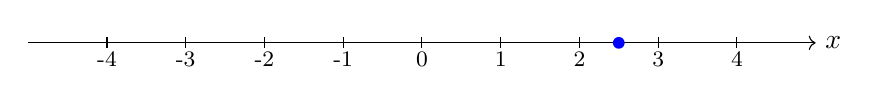
\begin{tikzpicture}
\draw[thin,->] (-5,0) -- (5,0) node[anchor=west] {$x$};
\foreach \x in {-4,-3,-2,-1,0,1,2,3,4}
\draw (\x cm,2pt) -- (\x cm,-2pt);
\foreach \x in {-4,-3,-2,-1,0,1,2,3,4}
\node[anchor=north] at (\x cm,0) {\footnotesize \x};
\node at (2.5 cm,0)[circle,fill,inner sep=1.5pt,color=blue] {};
\end{tikzpicture}



\begin{tikzpicture}
\draw[thin,->] (-5,0) -- (5,0) node[anchor=west] {$x$};
\foreach \x in {-4,-3,-2,-1,0,1,2,3,4}
\draw (\x cm,2pt) -- (\x cm,-2pt);
\foreach \x in {-4,-3,-2,-1,1,2,3,4}
\node[anchor=north] at (\x cm,0) {\footnotesize \x};
\draw[thin,->] (0,-5) -- (0,5) node[anchor=south] {$y$};
\foreach \y in {-4,-3,-2,-1,0,1,2,3,4}
\draw (2pt, \y cm) -- (-2pt, \y cm);
\foreach \y in {-4,-3,-2,-1,1,2,3,4}
\node[anchor=west] at (0, \y cm) {\footnotesize \y};
\node[anchor=north west] at (0,0) {\footnotesize O};
 \draw[thin,color=blue] (-3,-5) -- (5,4); ;
\end{tikzpicture}
 


\newpage

 $ S:= \{(1,1), (1,2), (1,3)\}  \subset \mathbb{R}^2 $  
\sep


















A line, defined by  points $(x,y)$ in the plane 



\clearpage


\subsection{Notation: Sets}


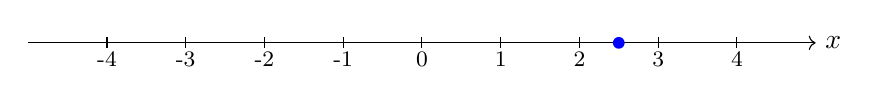
\begin{tikzpicture}
\draw[thin,->] (-5,0) -- (5,0) node[anchor=west] {$x$};
\foreach \x in {-4,-3,-2,-1,0,1,2,3,4}
\draw (\x cm,2pt) -- (\x cm,-2pt);
\foreach \x in {-4,-3,-2,-1,0,1,2,3,4}
\node[anchor=north] at (\x cm,0) {\footnotesize \x};
\node at (2.5 cm,0)[circle,fill,inner sep=1.5pt,color=blue] {};
\end{tikzpicture}



\begin{tikzpicture}
\draw[thin,->] (-5,0) -- (5,0) node[anchor=west] {$x$};
\foreach \x in {-4,-3,-2,-1,0,1,2,3,4}
\draw (\x cm,2pt) -- (\x cm,-2pt);
\foreach \x in {-4,-3,-2,-1,1,2,3,4}
\node[anchor=north] at (\x cm,0) {\footnotesize \x};
\draw[thin,->] (0,-5) -- (0,5) node[anchor=south] {$y$};
\foreach \y in {-4,-3,-2,-1,0,1,2,3,4}
\draw (2pt, \y cm) -- (-2pt, \y cm);
\foreach \y in {-4,-3,-2,-1,1,2,3,4}
\node[anchor=west] at (0, \y cm) {\footnotesize \y};
\node[anchor=north west] at (0,0) {\footnotesize O};
 \draw[thin,color=blue] (-3,-5) -- (5,4); ;
\end{tikzpicture}
 


\newpage

 $ S:= \{(1,1), (1,2), (1,3)\}  \subset \mathbb{R}^2 $  
\sep


















A line, defined by  points $(x,y)$ in the plane  so that $y = x - 1.7$ 



\clearpage


\subsection{Notation: Sets}


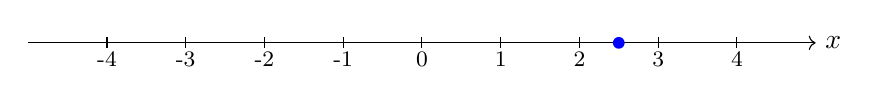
\begin{tikzpicture}
\draw[thin,->] (-5,0) -- (5,0) node[anchor=west] {$x$};
\foreach \x in {-4,-3,-2,-1,0,1,2,3,4}
\draw (\x cm,2pt) -- (\x cm,-2pt);
\foreach \x in {-4,-3,-2,-1,0,1,2,3,4}
\node[anchor=north] at (\x cm,0) {\footnotesize \x};
\node at (2.5 cm,0)[circle,fill,inner sep=1.5pt,color=blue] {};
\end{tikzpicture}



\begin{tikzpicture}
\draw[thin,->] (-5,0) -- (5,0) node[anchor=west] {$x$};
\foreach \x in {-4,-3,-2,-1,0,1,2,3,4}
\draw (\x cm,2pt) -- (\x cm,-2pt);
\foreach \x in {-4,-3,-2,-1,1,2,3,4}
\node[anchor=north] at (\x cm,0) {\footnotesize \x};
\draw[thin,->] (0,-5) -- (0,5) node[anchor=south] {$y$};
\foreach \y in {-4,-3,-2,-1,0,1,2,3,4}
\draw (2pt, \y cm) -- (-2pt, \y cm);
\foreach \y in {-4,-3,-2,-1,1,2,3,4}
\node[anchor=west] at (0, \y cm) {\footnotesize \y};
\node[anchor=north west] at (0,0) {\footnotesize O};
 \draw[thin,color=blue] (-3,-5) -- (5,4); ;
\end{tikzpicture}
 


\newpage

 $ S:= \{(1,1), (1,2), (1,3)\}  \subset \mathbb{R}^2 $  
\sep


















A line, defined by  points $(x,y)$ in the plane  so that $y = x - 1.7$ 


$\{???\}$




\clearpage


\subsection{Notation: Sets}


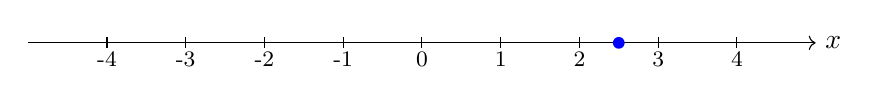
\begin{tikzpicture}
\draw[thin,->] (-5,0) -- (5,0) node[anchor=west] {$x$};
\foreach \x in {-4,-3,-2,-1,0,1,2,3,4}
\draw (\x cm,2pt) -- (\x cm,-2pt);
\foreach \x in {-4,-3,-2,-1,0,1,2,3,4}
\node[anchor=north] at (\x cm,0) {\footnotesize \x};
\node at (2.5 cm,0)[circle,fill,inner sep=1.5pt,color=blue] {};
\end{tikzpicture}



\begin{tikzpicture}
\draw[thin,->] (-5,0) -- (5,0) node[anchor=west] {$x$};
\foreach \x in {-4,-3,-2,-1,0,1,2,3,4}
\draw (\x cm,2pt) -- (\x cm,-2pt);
\foreach \x in {-4,-3,-2,-1,1,2,3,4}
\node[anchor=north] at (\x cm,0) {\footnotesize \x};
\draw[thin,->] (0,-5) -- (0,5) node[anchor=south] {$y$};
\foreach \y in {-4,-3,-2,-1,0,1,2,3,4}
\draw (2pt, \y cm) -- (-2pt, \y cm);
\foreach \y in {-4,-3,-2,-1,1,2,3,4}
\node[anchor=west] at (0, \y cm) {\footnotesize \y};
\node[anchor=north west] at (0,0) {\footnotesize O};
 \draw[thin,color=blue] (-3,-5) -- (5,4); ;
\end{tikzpicture}
 


\newpage

 $ S:= \{(1,1), (1,2), (1,3)\}  \subset \mathbb{R}^2 $  
\sep


















A line, defined by  \alert{points $(x,y)$} in the plane  so that $y = x - 1.7$ 


$\{(x,y) \}$




\clearpage


\subsection{Notation: Sets}


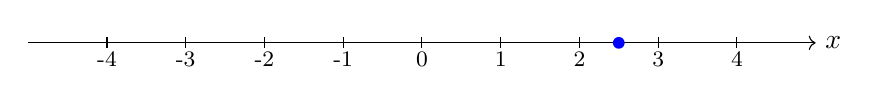
\begin{tikzpicture}
\draw[thin,->] (-5,0) -- (5,0) node[anchor=west] {$x$};
\foreach \x in {-4,-3,-2,-1,0,1,2,3,4}
\draw (\x cm,2pt) -- (\x cm,-2pt);
\foreach \x in {-4,-3,-2,-1,0,1,2,3,4}
\node[anchor=north] at (\x cm,0) {\footnotesize \x};
\node at (2.5 cm,0)[circle,fill,inner sep=1.5pt,color=blue] {};
\end{tikzpicture}



\begin{tikzpicture}
\draw[thin,->] (-5,0) -- (5,0) node[anchor=west] {$x$};
\foreach \x in {-4,-3,-2,-1,0,1,2,3,4}
\draw (\x cm,2pt) -- (\x cm,-2pt);
\foreach \x in {-4,-3,-2,-1,1,2,3,4}
\node[anchor=north] at (\x cm,0) {\footnotesize \x};
\draw[thin,->] (0,-5) -- (0,5) node[anchor=south] {$y$};
\foreach \y in {-4,-3,-2,-1,0,1,2,3,4}
\draw (2pt, \y cm) -- (-2pt, \y cm);
\foreach \y in {-4,-3,-2,-1,1,2,3,4}
\node[anchor=west] at (0, \y cm) {\footnotesize \y};
\node[anchor=north west] at (0,0) {\footnotesize O};
 \draw[thin,color=blue] (-3,-5) -- (5,4); ;
\end{tikzpicture}
 


\newpage

 $ S:= \{(1,1), (1,2), (1,3)\}  \subset \mathbb{R}^2 $  
\sep


















A line, defined by  \alert{points $(x,y)$} \alert{in the plane}  so that $y = x - 1.7$ 


$\{(x,y) \in \mathbb{R}^2 \}$




\clearpage


\subsection{Notation: Sets}


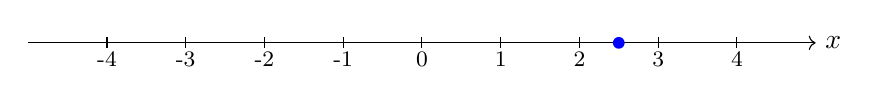
\begin{tikzpicture}
\draw[thin,->] (-5,0) -- (5,0) node[anchor=west] {$x$};
\foreach \x in {-4,-3,-2,-1,0,1,2,3,4}
\draw (\x cm,2pt) -- (\x cm,-2pt);
\foreach \x in {-4,-3,-2,-1,0,1,2,3,4}
\node[anchor=north] at (\x cm,0) {\footnotesize \x};
\node at (2.5 cm,0)[circle,fill,inner sep=1.5pt,color=blue] {};
\end{tikzpicture}



\begin{tikzpicture}
\draw[thin,->] (-5,0) -- (5,0) node[anchor=west] {$x$};
\foreach \x in {-4,-3,-2,-1,0,1,2,3,4}
\draw (\x cm,2pt) -- (\x cm,-2pt);
\foreach \x in {-4,-3,-2,-1,1,2,3,4}
\node[anchor=north] at (\x cm,0) {\footnotesize \x};
\draw[thin,->] (0,-5) -- (0,5) node[anchor=south] {$y$};
\foreach \y in {-4,-3,-2,-1,0,1,2,3,4}
\draw (2pt, \y cm) -- (-2pt, \y cm);
\foreach \y in {-4,-3,-2,-1,1,2,3,4}
\node[anchor=west] at (0, \y cm) {\footnotesize \y};
\node[anchor=north west] at (0,0) {\footnotesize O};
 \draw[thin,color=blue] (-3,-5) -- (5,4); ;
\end{tikzpicture}
 


\newpage

 $ S:= \{(1,1), (1,2), (1,3)\}  \subset \mathbb{R}^2 $  
\sep


















A line, defined by  \alert{points $(x,y)$} \alert{in the plane}  \alert{so that} $y = x - 1.7$ 


$\{(x,y) \in \mathbb{R}^2 \ |\ \}$




\clearpage


\subsection{Notation: Sets}


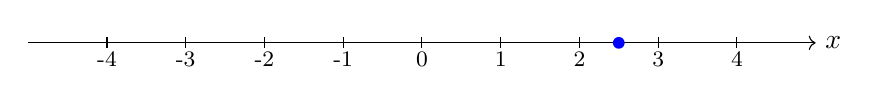
\begin{tikzpicture}
\draw[thin,->] (-5,0) -- (5,0) node[anchor=west] {$x$};
\foreach \x in {-4,-3,-2,-1,0,1,2,3,4}
\draw (\x cm,2pt) -- (\x cm,-2pt);
\foreach \x in {-4,-3,-2,-1,0,1,2,3,4}
\node[anchor=north] at (\x cm,0) {\footnotesize \x};
\node at (2.5 cm,0)[circle,fill,inner sep=1.5pt,color=blue] {};
\end{tikzpicture}



\begin{tikzpicture}
\draw[thin,->] (-5,0) -- (5,0) node[anchor=west] {$x$};
\foreach \x in {-4,-3,-2,-1,0,1,2,3,4}
\draw (\x cm,2pt) -- (\x cm,-2pt);
\foreach \x in {-4,-3,-2,-1,1,2,3,4}
\node[anchor=north] at (\x cm,0) {\footnotesize \x};
\draw[thin,->] (0,-5) -- (0,5) node[anchor=south] {$y$};
\foreach \y in {-4,-3,-2,-1,0,1,2,3,4}
\draw (2pt, \y cm) -- (-2pt, \y cm);
\foreach \y in {-4,-3,-2,-1,1,2,3,4}
\node[anchor=west] at (0, \y cm) {\footnotesize \y};
\node[anchor=north west] at (0,0) {\footnotesize O};
 \draw[thin,color=blue] (-3,-5) -- (5,4); ;
\end{tikzpicture}
 


\newpage

 $ S:= \{(1,1), (1,2), (1,3)\}  \subset \mathbb{R}^2 $  
\sep


















A line, defined by  \alert{points $(x,y)$} \alert{in the plane}  \alert{so that} \alert{$y = x - 1.7$} 


$\{(x,y) \in \mathbb{R}^2 \ |\ y = x - 1.75 \}$
 



\clearpage


\subsection{Notation: Sets}


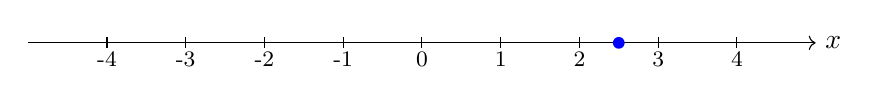
\begin{tikzpicture}
\draw[thin,->] (-5,0) -- (5,0) node[anchor=west] {$x$};
\foreach \x in {-4,-3,-2,-1,0,1,2,3,4}
\draw (\x cm,2pt) -- (\x cm,-2pt);
\foreach \x in {-4,-3,-2,-1,0,1,2,3,4}
\node[anchor=north] at (\x cm,0) {\footnotesize \x};
\node at (2.5 cm,0)[circle,fill,inner sep=1.5pt,color=blue] {};
\end{tikzpicture}



\begin{tikzpicture}
\draw[thin,->] (-5,0) -- (5,0) node[anchor=west] {$x$};
\foreach \x in {-4,-3,-2,-1,0,1,2,3,4}
\draw (\x cm,2pt) -- (\x cm,-2pt);
\foreach \x in {-4,-3,-2,-1,1,2,3,4}
\node[anchor=north] at (\x cm,0) {\footnotesize \x};
\draw[thin,->] (0,-5) -- (0,5) node[anchor=south] {$y$};
\foreach \y in {-4,-3,-2,-1,0,1,2,3,4}
\draw (2pt, \y cm) -- (-2pt, \y cm);
\foreach \y in {-4,-3,-2,-1,1,2,3,4}
\node[anchor=west] at (0, \y cm) {\footnotesize \y};
\node[anchor=north west] at (0,0) {\footnotesize O};
 \draw[thin,color=blue] (-3,-5) -- (5,4); ;
\end{tikzpicture}
 


\newpage

 $ S:= \{(1,1), (1,2), (1,3)\}  \subset \mathbb{R}^2 $  
\sep


















A line, defined by  \alert{points $(x,y)$} \alert{in the plane}  \alert{so that} \alert{$y = x - 1.7$} 


$ C:= \{(x,y) \in \mathbb{R}^2 \ |\ y = x - 1.75 \}$
 

\sep





\clearpage


\subsection{Notation: Sets}


\begin{tikzpicture}
\draw[thin,->] (-5,0) -- (5,0) node[anchor=west] {$x$};
\foreach \x in {-4,-3,-2,-1,0,1,2,3,4}
\draw (\x cm,2pt) -- (\x cm,-2pt);
\foreach \x in {-4,-3,-2,-1,0,1,2,3,4}
\node[anchor=north] at (\x cm,0) {\footnotesize \x};
\node at (2.5 cm,0)[circle,fill,inner sep=1.5pt,color=blue] {};
\end{tikzpicture}



\begin{tikzpicture}
\draw[thin,->] (-5,0) -- (5,0) node[anchor=west] {$x$};
\foreach \x in {-4,-3,-2,-1,0,1,2,3,4}
\draw (\x cm,2pt) -- (\x cm,-2pt);
\foreach \x in {-4,-3,-2,-1,1,2,3,4}
\node[anchor=north] at (\x cm,0) {\footnotesize \x};
\draw[thin,->] (0,-5) -- (0,5) node[anchor=south] {$y$};
\foreach \y in {-4,-3,-2,-1,0,1,2,3,4}
\draw (2pt, \y cm) -- (-2pt, \y cm);
\foreach \y in {-4,-3,-2,-1,1,2,3,4}
\node[anchor=west] at (0, \y cm) {\footnotesize \y};
\node[anchor=north west] at (0,0) {\footnotesize O};
 \draw[thin,color=blue] (-3,-5) -- (5,4); ;
\end{tikzpicture}
 


\newpage

 $ S:= \{(1,1), (1,2), (1,3)\}  \subset \mathbb{R}^2 $  
\sep


















A line, defined by  \alert{points $(x,y)$} \alert{in the plane}  \alert{so that} \alert{$y = x - 1.7$} 


$ C:= \{(x,y) \in \mathbb{R}^2 \ |\ y = x - 1.75 \}$
 

\sep

\begin{examples}
\item $\mathbb{R}:$ set of all real numbers. $2, \pi \textrm{ etc } \in \mathbb{R}$
  \end{examples}



\clearpage


\subsection{Notation: Sets}


\begin{tikzpicture}
\draw[thin,->] (-5,0) -- (5,0) node[anchor=west] {$x$};
\foreach \x in {-4,-3,-2,-1,0,1,2,3,4}
\draw (\x cm,2pt) -- (\x cm,-2pt);
\foreach \x in {-4,-3,-2,-1,0,1,2,3,4}
\node[anchor=north] at (\x cm,0) {\footnotesize \x};
\node at (2.5 cm,0)[circle,fill,inner sep=1.5pt,color=blue] {};
\end{tikzpicture}



\begin{tikzpicture}
\draw[thin,->] (-5,0) -- (5,0) node[anchor=west] {$x$};
\foreach \x in {-4,-3,-2,-1,0,1,2,3,4}
\draw (\x cm,2pt) -- (\x cm,-2pt);
\foreach \x in {-4,-3,-2,-1,1,2,3,4}
\node[anchor=north] at (\x cm,0) {\footnotesize \x};
\draw[thin,->] (0,-5) -- (0,5) node[anchor=south] {$y$};
\foreach \y in {-4,-3,-2,-1,0,1,2,3,4}
\draw (2pt, \y cm) -- (-2pt, \y cm);
\foreach \y in {-4,-3,-2,-1,1,2,3,4}
\node[anchor=west] at (0, \y cm) {\footnotesize \y};
\node[anchor=north west] at (0,0) {\footnotesize O};
 \draw[thin,color=blue] (-3,-5) -- (5,4); ;
\end{tikzpicture}
 


\newpage

 $ S:= \{(1,1), (1,2), (1,3)\}  \subset \mathbb{R}^2 $  
\sep


















A line, defined by  \alert{points $(x,y)$} \alert{in the plane}  \alert{so that} \alert{$y = x - 1.7$} 


$ C:= \{(x,y) \in \mathbb{R}^2 \ |\ y = x - 1.75 \}$
 

\sep

\begin{examples}
\item $\mathbb{R}:$ set of all real numbers. $2, \pi \textrm{ etc } \in \mathbb{R}$
  \item $\{x \in \mathbb{R} \}$\end{examples}



\clearpage


\subsection{Notation: Sets}


\begin{tikzpicture}
\draw[thin,->] (-5,0) -- (5,0) node[anchor=west] {$x$};
\foreach \x in {-4,-3,-2,-1,0,1,2,3,4}
\draw (\x cm,2pt) -- (\x cm,-2pt);
\foreach \x in {-4,-3,-2,-1,0,1,2,3,4}
\node[anchor=north] at (\x cm,0) {\footnotesize \x};
\node at (2.5 cm,0)[circle,fill,inner sep=1.5pt,color=blue] {};
\end{tikzpicture}



\begin{tikzpicture}
\draw[thin,->] (-5,0) -- (5,0) node[anchor=west] {$x$};
\foreach \x in {-4,-3,-2,-1,0,1,2,3,4}
\draw (\x cm,2pt) -- (\x cm,-2pt);
\foreach \x in {-4,-3,-2,-1,1,2,3,4}
\node[anchor=north] at (\x cm,0) {\footnotesize \x};
\draw[thin,->] (0,-5) -- (0,5) node[anchor=south] {$y$};
\foreach \y in {-4,-3,-2,-1,0,1,2,3,4}
\draw (2pt, \y cm) -- (-2pt, \y cm);
\foreach \y in {-4,-3,-2,-1,1,2,3,4}
\node[anchor=west] at (0, \y cm) {\footnotesize \y};
\node[anchor=north west] at (0,0) {\footnotesize O};
 \draw[thin,color=blue] (-3,-5) -- (5,4); ;
\end{tikzpicture}
 


\newpage

 $ S:= \{(1,1), (1,2), (1,3)\}  \subset \mathbb{R}^2 $  
\sep


















A line, defined by  \alert{points $(x,y)$} \alert{in the plane}  \alert{so that} \alert{$y = x - 1.7$} 


$ C:= \{(x,y) \in \mathbb{R}^2 \ |\ y = x - 1.75 \}$
 

\sep

\begin{examples}
\item $\mathbb{R}:$ set of all real numbers. $2, \pi \textrm{ etc } \in \mathbb{R}$
  \item $\{x \in \mathbb{R} \ |\ \}$\end{examples}



\clearpage


\subsection{Notation: Sets}


\begin{tikzpicture}
\draw[thin,->] (-5,0) -- (5,0) node[anchor=west] {$x$};
\foreach \x in {-4,-3,-2,-1,0,1,2,3,4}
\draw (\x cm,2pt) -- (\x cm,-2pt);
\foreach \x in {-4,-3,-2,-1,0,1,2,3,4}
\node[anchor=north] at (\x cm,0) {\footnotesize \x};
\node at (2.5 cm,0)[circle,fill,inner sep=1.5pt,color=blue] {};
\end{tikzpicture}



\begin{tikzpicture}
\draw[thin,->] (-5,0) -- (5,0) node[anchor=west] {$x$};
\foreach \x in {-4,-3,-2,-1,0,1,2,3,4}
\draw (\x cm,2pt) -- (\x cm,-2pt);
\foreach \x in {-4,-3,-2,-1,1,2,3,4}
\node[anchor=north] at (\x cm,0) {\footnotesize \x};
\draw[thin,->] (0,-5) -- (0,5) node[anchor=south] {$y$};
\foreach \y in {-4,-3,-2,-1,0,1,2,3,4}
\draw (2pt, \y cm) -- (-2pt, \y cm);
\foreach \y in {-4,-3,-2,-1,1,2,3,4}
\node[anchor=west] at (0, \y cm) {\footnotesize \y};
\node[anchor=north west] at (0,0) {\footnotesize O};
 \draw[thin,color=blue] (-3,-5) -- (5,4); ;
\end{tikzpicture}
 


\newpage

 $ S:= \{(1,1), (1,2), (1,3)\}  \subset \mathbb{R}^2 $  
\sep


















A line, defined by  \alert{points $(x,y)$} \alert{in the plane}  \alert{so that} \alert{$y = x - 1.7$} 


$ C:= \{(x,y) \in \mathbb{R}^2 \ |\ y = x - 1.75 \}$
 

\sep

\begin{examples}
\item $\mathbb{R}:$ set of all real numbers. $2, \pi \textrm{ etc } \in \mathbb{R}$
  \item $\{x \in \mathbb{R} \ |\  \alpha < x \}$\end{examples}



\clearpage


\subsection{Notation: Sets}


\begin{tikzpicture}
\draw[thin,->] (-5,0) -- (5,0) node[anchor=west] {$x$};
\foreach \x in {-4,-3,-2,-1,0,1,2,3,4}
\draw (\x cm,2pt) -- (\x cm,-2pt);
\foreach \x in {-4,-3,-2,-1,0,1,2,3,4}
\node[anchor=north] at (\x cm,0) {\footnotesize \x};
\node at (2.5 cm,0)[circle,fill,inner sep=1.5pt,color=blue] {};
\end{tikzpicture}



\begin{tikzpicture}
\draw[thin,->] (-5,0) -- (5,0) node[anchor=west] {$x$};
\foreach \x in {-4,-3,-2,-1,0,1,2,3,4}
\draw (\x cm,2pt) -- (\x cm,-2pt);
\foreach \x in {-4,-3,-2,-1,1,2,3,4}
\node[anchor=north] at (\x cm,0) {\footnotesize \x};
\draw[thin,->] (0,-5) -- (0,5) node[anchor=south] {$y$};
\foreach \y in {-4,-3,-2,-1,0,1,2,3,4}
\draw (2pt, \y cm) -- (-2pt, \y cm);
\foreach \y in {-4,-3,-2,-1,1,2,3,4}
\node[anchor=west] at (0, \y cm) {\footnotesize \y};
\node[anchor=north west] at (0,0) {\footnotesize O};
 \draw[thin,color=blue] (-3,-5) -- (5,4); ;
\end{tikzpicture}
 


\newpage

 $ S:= \{(1,1), (1,2), (1,3)\}  \subset \mathbb{R}^2 $  
\sep


















A line, defined by  \alert{points $(x,y)$} \alert{in the plane}  \alert{so that} \alert{$y = x - 1.7$} 


$ C:= \{(x,y) \in \mathbb{R}^2 \ |\ y = x - 1.75 \}$
 

\sep

\begin{examples}
\item $\mathbb{R}:$ set of all real numbers. $2, \pi \textrm{ etc } \in \mathbb{R}$
  \item $\{x \in \mathbb{R} \ |\  \alpha < x  < \beta \}$
  \end{examples}



\clearpage


\subsection{Notation: Sets}


\begin{tikzpicture}
\draw[thin,->] (-5,0) -- (5,0) node[anchor=west] {$x$};
\foreach \x in {-4,-3,-2,-1,0,1,2,3,4}
\draw (\x cm,2pt) -- (\x cm,-2pt);
\foreach \x in {-4,-3,-2,-1,0,1,2,3,4}
\node[anchor=north] at (\x cm,0) {\footnotesize \x};
\node at (2.5 cm,0)[circle,fill,inner sep=1.5pt,color=blue] {};
\end{tikzpicture}



\begin{tikzpicture}
\draw[thin,->] (-5,0) -- (5,0) node[anchor=west] {$x$};
\foreach \x in {-4,-3,-2,-1,0,1,2,3,4}
\draw (\x cm,2pt) -- (\x cm,-2pt);
\foreach \x in {-4,-3,-2,-1,1,2,3,4}
\node[anchor=north] at (\x cm,0) {\footnotesize \x};
\draw[thin,->] (0,-5) -- (0,5) node[anchor=south] {$y$};
\foreach \y in {-4,-3,-2,-1,0,1,2,3,4}
\draw (2pt, \y cm) -- (-2pt, \y cm);
\foreach \y in {-4,-3,-2,-1,1,2,3,4}
\node[anchor=west] at (0, \y cm) {\footnotesize \y};
\node[anchor=north west] at (0,0) {\footnotesize O};
 \draw[thin,color=blue] (-3,-5) -- (5,4); ;
\end{tikzpicture}
 


\newpage

 $ S:= \{(1,1), (1,2), (1,3)\}  \subset \mathbb{R}^2 $  
\sep


















A line, defined by  \alert{points $(x,y)$} \alert{in the plane}  \alert{so that} \alert{$y = x - 1.7$} 


$ C:= \{(x,y) \in \mathbb{R}^2 \ |\ y = x - 1.75 \}$
 

\sep

\begin{examples}
\item $\mathbb{R}:$ set of all real numbers. $2, \pi \textrm{ etc } \in \mathbb{R}$
  \item $ := \{x \in \mathbb{R} \ |\  \alpha < x  < \beta \}$
  
  \end{examples}



\clearpage


\subsection{Notation: Sets}


\begin{tikzpicture}
\draw[thin,->] (-5,0) -- (5,0) node[anchor=west] {$x$};
\foreach \x in {-4,-3,-2,-1,0,1,2,3,4}
\draw (\x cm,2pt) -- (\x cm,-2pt);
\foreach \x in {-4,-3,-2,-1,0,1,2,3,4}
\node[anchor=north] at (\x cm,0) {\footnotesize \x};
\node at (2.5 cm,0)[circle,fill,inner sep=1.5pt,color=blue] {};
\end{tikzpicture}



\begin{tikzpicture}
\draw[thin,->] (-5,0) -- (5,0) node[anchor=west] {$x$};
\foreach \x in {-4,-3,-2,-1,0,1,2,3,4}
\draw (\x cm,2pt) -- (\x cm,-2pt);
\foreach \x in {-4,-3,-2,-1,1,2,3,4}
\node[anchor=north] at (\x cm,0) {\footnotesize \x};
\draw[thin,->] (0,-5) -- (0,5) node[anchor=south] {$y$};
\foreach \y in {-4,-3,-2,-1,0,1,2,3,4}
\draw (2pt, \y cm) -- (-2pt, \y cm);
\foreach \y in {-4,-3,-2,-1,1,2,3,4}
\node[anchor=west] at (0, \y cm) {\footnotesize \y};
\node[anchor=north west] at (0,0) {\footnotesize O};
 \draw[thin,color=blue] (-3,-5) -- (5,4); ;
\end{tikzpicture}
 


\newpage

 $ S:= \{(1,1), (1,2), (1,3)\}  \subset \mathbb{R}^2 $  
\sep


















A line, defined by  \alert{points $(x,y)$} \alert{in the plane}  \alert{so that} \alert{$y = x - 1.7$} 


$ C:= \{(x,y) \in \mathbb{R}^2 \ |\ y = x - 1.75 \}$
 

\sep

\begin{examples}
\item $\mathbb{R}:$ set of all real numbers. $2, \pi \textrm{ etc } \in \mathbb{R}$
  \item $ (\alpha,  := \{x \in \mathbb{R} \ |\  \alpha < x  < \beta \}$
  
  \end{examples}



\clearpage


\subsection{Notation: Sets}


\begin{tikzpicture}
\draw[thin,->] (-5,0) -- (5,0) node[anchor=west] {$x$};
\foreach \x in {-4,-3,-2,-1,0,1,2,3,4}
\draw (\x cm,2pt) -- (\x cm,-2pt);
\foreach \x in {-4,-3,-2,-1,0,1,2,3,4}
\node[anchor=north] at (\x cm,0) {\footnotesize \x};
\node at (2.5 cm,0)[circle,fill,inner sep=1.5pt,color=blue] {};
\end{tikzpicture}



\begin{tikzpicture}
\draw[thin,->] (-5,0) -- (5,0) node[anchor=west] {$x$};
\foreach \x in {-4,-3,-2,-1,0,1,2,3,4}
\draw (\x cm,2pt) -- (\x cm,-2pt);
\foreach \x in {-4,-3,-2,-1,1,2,3,4}
\node[anchor=north] at (\x cm,0) {\footnotesize \x};
\draw[thin,->] (0,-5) -- (0,5) node[anchor=south] {$y$};
\foreach \y in {-4,-3,-2,-1,0,1,2,3,4}
\draw (2pt, \y cm) -- (-2pt, \y cm);
\foreach \y in {-4,-3,-2,-1,1,2,3,4}
\node[anchor=west] at (0, \y cm) {\footnotesize \y};
\node[anchor=north west] at (0,0) {\footnotesize O};
 \draw[thin,color=blue] (-3,-5) -- (5,4); ;
\end{tikzpicture}
 


\newpage

 $ S:= \{(1,1), (1,2), (1,3)\}  \subset \mathbb{R}^2 $  
\sep


















A line, defined by  \alert{points $(x,y)$} \alert{in the plane}  \alert{so that} \alert{$y = x - 1.7$} 


$ C:= \{(x,y) \in \mathbb{R}^2 \ |\ y = x - 1.75 \}$
 

\sep

\begin{examples}
\item $\mathbb{R}:$ set of all real numbers. $2, \pi \textrm{ etc } \in \mathbb{R}$
  \item $ (\alpha,  \beta) := \{x \in \mathbb{R} \ |\  \alpha < x  < \beta \}$
  
  
  \end{examples}



\clearpage


\subsection{Notation: Sets}


\begin{tikzpicture}
\draw[thin,->] (-5,0) -- (5,0) node[anchor=west] {$x$};
\foreach \x in {-4,-3,-2,-1,0,1,2,3,4}
\draw (\x cm,2pt) -- (\x cm,-2pt);
\foreach \x in {-4,-3,-2,-1,0,1,2,3,4}
\node[anchor=north] at (\x cm,0) {\footnotesize \x};
\node at (2.5 cm,0)[circle,fill,inner sep=1.5pt,color=blue] {};
\end{tikzpicture}



\begin{tikzpicture}
\draw[thin,->] (-5,0) -- (5,0) node[anchor=west] {$x$};
\foreach \x in {-4,-3,-2,-1,0,1,2,3,4}
\draw (\x cm,2pt) -- (\x cm,-2pt);
\foreach \x in {-4,-3,-2,-1,1,2,3,4}
\node[anchor=north] at (\x cm,0) {\footnotesize \x};
\draw[thin,->] (0,-5) -- (0,5) node[anchor=south] {$y$};
\foreach \y in {-4,-3,-2,-1,0,1,2,3,4}
\draw (2pt, \y cm) -- (-2pt, \y cm);
\foreach \y in {-4,-3,-2,-1,1,2,3,4}
\node[anchor=west] at (0, \y cm) {\footnotesize \y};
\node[anchor=north west] at (0,0) {\footnotesize O};
 \draw[thin,color=blue] (-3,-5) -- (5,4); ;
\end{tikzpicture}
 


\newpage

 $ S:= \{(1,1), (1,2), (1,3)\}  \subset \mathbb{R}^2 $  
\sep


















A line, defined by  \alert{points $(x,y)$} \alert{in the plane}  \alert{so that} \alert{$y = x - 1.7$} 


$ C:= \{(x,y) \in \mathbb{R}^2 \ |\ y = x - 1.75 \}$
 

\sep

\begin{examples}
\item $\mathbb{R}:$ set of all real numbers. $2, \pi \textrm{ etc } \in \mathbb{R}$
  \item $ (\alpha,  \beta) := \{x \in \mathbb{R} \ |\  \alpha < x  < \beta \}$
  
  
  \item $\{x \in \mathbb{R} \}$\end{examples}



\clearpage


\subsection{Notation: Sets}


\begin{tikzpicture}
\draw[thin,->] (-5,0) -- (5,0) node[anchor=west] {$x$};
\foreach \x in {-4,-3,-2,-1,0,1,2,3,4}
\draw (\x cm,2pt) -- (\x cm,-2pt);
\foreach \x in {-4,-3,-2,-1,0,1,2,3,4}
\node[anchor=north] at (\x cm,0) {\footnotesize \x};
\node at (2.5 cm,0)[circle,fill,inner sep=1.5pt,color=blue] {};
\end{tikzpicture}



\begin{tikzpicture}
\draw[thin,->] (-5,0) -- (5,0) node[anchor=west] {$x$};
\foreach \x in {-4,-3,-2,-1,0,1,2,3,4}
\draw (\x cm,2pt) -- (\x cm,-2pt);
\foreach \x in {-4,-3,-2,-1,1,2,3,4}
\node[anchor=north] at (\x cm,0) {\footnotesize \x};
\draw[thin,->] (0,-5) -- (0,5) node[anchor=south] {$y$};
\foreach \y in {-4,-3,-2,-1,0,1,2,3,4}
\draw (2pt, \y cm) -- (-2pt, \y cm);
\foreach \y in {-4,-3,-2,-1,1,2,3,4}
\node[anchor=west] at (0, \y cm) {\footnotesize \y};
\node[anchor=north west] at (0,0) {\footnotesize O};
 \draw[thin,color=blue] (-3,-5) -- (5,4); ;
\end{tikzpicture}
 


\newpage

 $ S:= \{(1,1), (1,2), (1,3)\}  \subset \mathbb{R}^2 $  
\sep


















A line, defined by  \alert{points $(x,y)$} \alert{in the plane}  \alert{so that} \alert{$y = x - 1.7$} 


$ C:= \{(x,y) \in \mathbb{R}^2 \ |\ y = x - 1.75 \}$
 

\sep

\begin{examples}
\item $\mathbb{R}:$ set of all real numbers. $2, \pi \textrm{ etc } \in \mathbb{R}$
  \item $ (\alpha,  \beta) := \{x \in \mathbb{R} \ |\  \alpha < x  < \beta \}$
  
  
  \item $\{x \in \mathbb{R} \ |\ \}$\end{examples}



\clearpage


\subsection{Notation: Sets}


\begin{tikzpicture}
\draw[thin,->] (-5,0) -- (5,0) node[anchor=west] {$x$};
\foreach \x in {-4,-3,-2,-1,0,1,2,3,4}
\draw (\x cm,2pt) -- (\x cm,-2pt);
\foreach \x in {-4,-3,-2,-1,0,1,2,3,4}
\node[anchor=north] at (\x cm,0) {\footnotesize \x};
\node at (2.5 cm,0)[circle,fill,inner sep=1.5pt,color=blue] {};
\end{tikzpicture}



\begin{tikzpicture}
\draw[thin,->] (-5,0) -- (5,0) node[anchor=west] {$x$};
\foreach \x in {-4,-3,-2,-1,0,1,2,3,4}
\draw (\x cm,2pt) -- (\x cm,-2pt);
\foreach \x in {-4,-3,-2,-1,1,2,3,4}
\node[anchor=north] at (\x cm,0) {\footnotesize \x};
\draw[thin,->] (0,-5) -- (0,5) node[anchor=south] {$y$};
\foreach \y in {-4,-3,-2,-1,0,1,2,3,4}
\draw (2pt, \y cm) -- (-2pt, \y cm);
\foreach \y in {-4,-3,-2,-1,1,2,3,4}
\node[anchor=west] at (0, \y cm) {\footnotesize \y};
\node[anchor=north west] at (0,0) {\footnotesize O};
 \draw[thin,color=blue] (-3,-5) -- (5,4); ;
\end{tikzpicture}
 


\newpage

 $ S:= \{(1,1), (1,2), (1,3)\}  \subset \mathbb{R}^2 $  
\sep


















A line, defined by  \alert{points $(x,y)$} \alert{in the plane}  \alert{so that} \alert{$y = x - 1.7$} 


$ C:= \{(x,y) \in \mathbb{R}^2 \ |\ y = x - 1.75 \}$
 

\sep

\begin{examples}
\item $\mathbb{R}:$ set of all real numbers. $2, \pi \textrm{ etc } \in \mathbb{R}$
  \item $ (\alpha,  \beta) := \{x \in \mathbb{R} \ |\  \alpha < x  < \beta \}$
  
  
  \item $\{x \in \mathbb{R} \ |\  \alpha < x \}$\end{examples}



\clearpage


\subsection{Notation: Sets}


\begin{tikzpicture}
\draw[thin,->] (-5,0) -- (5,0) node[anchor=west] {$x$};
\foreach \x in {-4,-3,-2,-1,0,1,2,3,4}
\draw (\x cm,2pt) -- (\x cm,-2pt);
\foreach \x in {-4,-3,-2,-1,0,1,2,3,4}
\node[anchor=north] at (\x cm,0) {\footnotesize \x};
\node at (2.5 cm,0)[circle,fill,inner sep=1.5pt,color=blue] {};
\end{tikzpicture}



\begin{tikzpicture}
\draw[thin,->] (-5,0) -- (5,0) node[anchor=west] {$x$};
\foreach \x in {-4,-3,-2,-1,0,1,2,3,4}
\draw (\x cm,2pt) -- (\x cm,-2pt);
\foreach \x in {-4,-3,-2,-1,1,2,3,4}
\node[anchor=north] at (\x cm,0) {\footnotesize \x};
\draw[thin,->] (0,-5) -- (0,5) node[anchor=south] {$y$};
\foreach \y in {-4,-3,-2,-1,0,1,2,3,4}
\draw (2pt, \y cm) -- (-2pt, \y cm);
\foreach \y in {-4,-3,-2,-1,1,2,3,4}
\node[anchor=west] at (0, \y cm) {\footnotesize \y};
\node[anchor=north west] at (0,0) {\footnotesize O};
 \draw[thin,color=blue] (-3,-5) -- (5,4); ;
\end{tikzpicture}
 


\newpage

 $ S:= \{(1,1), (1,2), (1,3)\}  \subset \mathbb{R}^2 $  
\sep


















A line, defined by  \alert{points $(x,y)$} \alert{in the plane}  \alert{so that} \alert{$y = x - 1.7$} 


$ C:= \{(x,y) \in \mathbb{R}^2 \ |\ y = x - 1.75 \}$
 

\sep

\begin{examples}
\item $\mathbb{R}:$ set of all real numbers. $2, \pi \textrm{ etc } \in \mathbb{R}$
  \item $ (\alpha,  \beta) := \{x \in \mathbb{R} \ |\  \alpha < x  < \beta \}$
  
  
  \item $\{x \in \mathbb{R} \ |\  \alpha < x  \leq \beta \}$
  \end{examples}



\clearpage


\subsection{Notation: Sets}


\begin{tikzpicture}
\draw[thin,->] (-5,0) -- (5,0) node[anchor=west] {$x$};
\foreach \x in {-4,-3,-2,-1,0,1,2,3,4}
\draw (\x cm,2pt) -- (\x cm,-2pt);
\foreach \x in {-4,-3,-2,-1,0,1,2,3,4}
\node[anchor=north] at (\x cm,0) {\footnotesize \x};
\node at (2.5 cm,0)[circle,fill,inner sep=1.5pt,color=blue] {};
\end{tikzpicture}



\begin{tikzpicture}
\draw[thin,->] (-5,0) -- (5,0) node[anchor=west] {$x$};
\foreach \x in {-4,-3,-2,-1,0,1,2,3,4}
\draw (\x cm,2pt) -- (\x cm,-2pt);
\foreach \x in {-4,-3,-2,-1,1,2,3,4}
\node[anchor=north] at (\x cm,0) {\footnotesize \x};
\draw[thin,->] (0,-5) -- (0,5) node[anchor=south] {$y$};
\foreach \y in {-4,-3,-2,-1,0,1,2,3,4}
\draw (2pt, \y cm) -- (-2pt, \y cm);
\foreach \y in {-4,-3,-2,-1,1,2,3,4}
\node[anchor=west] at (0, \y cm) {\footnotesize \y};
\node[anchor=north west] at (0,0) {\footnotesize O};
 \draw[thin,color=blue] (-3,-5) -- (5,4); ;
\end{tikzpicture}
 


\newpage

 $ S:= \{(1,1), (1,2), (1,3)\}  \subset \mathbb{R}^2 $  
\sep


















A line, defined by  \alert{points $(x,y)$} \alert{in the plane}  \alert{so that} \alert{$y = x - 1.7$} 


$ C:= \{(x,y) \in \mathbb{R}^2 \ |\ y = x - 1.75 \}$
 

\sep

\begin{examples}
\item $\mathbb{R}:$ set of all real numbers. $2, \pi \textrm{ etc } \in \mathbb{R}$
  \item $ (\alpha,  \beta) := \{x \in \mathbb{R} \ |\  \alpha < x  < \beta \}$
  
  
  \item $ := \{x \in \mathbb{R} \ |\  \alpha < x  \leq \beta \}$
  
  \end{examples}



\clearpage


\subsection{Notation: Sets}


\begin{tikzpicture}
\draw[thin,->] (-5,0) -- (5,0) node[anchor=west] {$x$};
\foreach \x in {-4,-3,-2,-1,0,1,2,3,4}
\draw (\x cm,2pt) -- (\x cm,-2pt);
\foreach \x in {-4,-3,-2,-1,0,1,2,3,4}
\node[anchor=north] at (\x cm,0) {\footnotesize \x};
\node at (2.5 cm,0)[circle,fill,inner sep=1.5pt,color=blue] {};
\end{tikzpicture}



\begin{tikzpicture}
\draw[thin,->] (-5,0) -- (5,0) node[anchor=west] {$x$};
\foreach \x in {-4,-3,-2,-1,0,1,2,3,4}
\draw (\x cm,2pt) -- (\x cm,-2pt);
\foreach \x in {-4,-3,-2,-1,1,2,3,4}
\node[anchor=north] at (\x cm,0) {\footnotesize \x};
\draw[thin,->] (0,-5) -- (0,5) node[anchor=south] {$y$};
\foreach \y in {-4,-3,-2,-1,0,1,2,3,4}
\draw (2pt, \y cm) -- (-2pt, \y cm);
\foreach \y in {-4,-3,-2,-1,1,2,3,4}
\node[anchor=west] at (0, \y cm) {\footnotesize \y};
\node[anchor=north west] at (0,0) {\footnotesize O};
 \draw[thin,color=blue] (-3,-5) -- (5,4); ;
\end{tikzpicture}
 


\newpage

 $ S:= \{(1,1), (1,2), (1,3)\}  \subset \mathbb{R}^2 $  
\sep


















A line, defined by  \alert{points $(x,y)$} \alert{in the plane}  \alert{so that} \alert{$y = x - 1.7$} 


$ C:= \{(x,y) \in \mathbb{R}^2 \ |\ y = x - 1.75 \}$
 

\sep

\begin{examples}
\item $\mathbb{R}:$ set of all real numbers. $2, \pi \textrm{ etc } \in \mathbb{R}$
  \item $ (\alpha,  \beta) := \{x \in \mathbb{R} \ |\  \alpha < x  < \beta \}$
  
  
  \item $ (\alpha,  := \{x \in \mathbb{R} \ |\  \alpha < x  \leq \beta \}$
  
  \end{examples}



\clearpage


\subsection{Notation: Sets}


\begin{tikzpicture}
\draw[thin,->] (-5,0) -- (5,0) node[anchor=west] {$x$};
\foreach \x in {-4,-3,-2,-1,0,1,2,3,4}
\draw (\x cm,2pt) -- (\x cm,-2pt);
\foreach \x in {-4,-3,-2,-1,0,1,2,3,4}
\node[anchor=north] at (\x cm,0) {\footnotesize \x};
\node at (2.5 cm,0)[circle,fill,inner sep=1.5pt,color=blue] {};
\end{tikzpicture}



\begin{tikzpicture}
\draw[thin,->] (-5,0) -- (5,0) node[anchor=west] {$x$};
\foreach \x in {-4,-3,-2,-1,0,1,2,3,4}
\draw (\x cm,2pt) -- (\x cm,-2pt);
\foreach \x in {-4,-3,-2,-1,1,2,3,4}
\node[anchor=north] at (\x cm,0) {\footnotesize \x};
\draw[thin,->] (0,-5) -- (0,5) node[anchor=south] {$y$};
\foreach \y in {-4,-3,-2,-1,0,1,2,3,4}
\draw (2pt, \y cm) -- (-2pt, \y cm);
\foreach \y in {-4,-3,-2,-1,1,2,3,4}
\node[anchor=west] at (0, \y cm) {\footnotesize \y};
\node[anchor=north west] at (0,0) {\footnotesize O};
 \draw[thin,color=blue] (-3,-5) -- (5,4); ;
\end{tikzpicture}
 


\newpage

 $ S:= \{(1,1), (1,2), (1,3)\}  \subset \mathbb{R}^2 $  
\sep


















A line, defined by  \alert{points $(x,y)$} \alert{in the plane}  \alert{so that} \alert{$y = x - 1.7$} 


$ C:= \{(x,y) \in \mathbb{R}^2 \ |\ y = x - 1.75 \}$
 

\sep

\begin{examples}
\item $\mathbb{R}:$ set of all real numbers. $2, \pi \textrm{ etc } \in \mathbb{R}$
  \item $ (\alpha,  \beta) := \{x \in \mathbb{R} \ |\  \alpha < x  < \beta \}$
  
  
  \item $ (\alpha,  \beta] := \{x \in \mathbb{R} \ |\  \alpha < x  \leq \beta \}$
  
  
  \end{examples}



\clearpage


\subsection{Notation: Sets}


\begin{tikzpicture}
\draw[thin,->] (-5,0) -- (5,0) node[anchor=west] {$x$};
\foreach \x in {-4,-3,-2,-1,0,1,2,3,4}
\draw (\x cm,2pt) -- (\x cm,-2pt);
\foreach \x in {-4,-3,-2,-1,0,1,2,3,4}
\node[anchor=north] at (\x cm,0) {\footnotesize \x};
\node at (2.5 cm,0)[circle,fill,inner sep=1.5pt,color=blue] {};
\end{tikzpicture}



\begin{tikzpicture}
\draw[thin,->] (-5,0) -- (5,0) node[anchor=west] {$x$};
\foreach \x in {-4,-3,-2,-1,0,1,2,3,4}
\draw (\x cm,2pt) -- (\x cm,-2pt);
\foreach \x in {-4,-3,-2,-1,1,2,3,4}
\node[anchor=north] at (\x cm,0) {\footnotesize \x};
\draw[thin,->] (0,-5) -- (0,5) node[anchor=south] {$y$};
\foreach \y in {-4,-3,-2,-1,0,1,2,3,4}
\draw (2pt, \y cm) -- (-2pt, \y cm);
\foreach \y in {-4,-3,-2,-1,1,2,3,4}
\node[anchor=west] at (0, \y cm) {\footnotesize \y};
\node[anchor=north west] at (0,0) {\footnotesize O};
 \draw[thin,color=blue] (-3,-5) -- (5,4); ;
\end{tikzpicture}
 


\newpage

 $ S:= \{(1,1), (1,2), (1,3)\}  \subset \mathbb{R}^2 $  
\sep


















A line, defined by  \alert{points $(x,y)$} \alert{in the plane}  \alert{so that} \alert{$y = x - 1.7$} 


$ C:= \{(x,y) \in \mathbb{R}^2 \ |\ y = x - 1.75 \}$
 

\sep

\begin{examples}
\item $\mathbb{R}:$ set of all real numbers. $2, \pi \textrm{ etc } \in \mathbb{R}$
  \item $ (\alpha,  \beta) := \{x \in \mathbb{R} \ |\  \alpha < x  < \beta \}$
  
  
  \item $ (\alpha,  \beta] := \{x \in \mathbb{R} \ |\  \alpha < x  \leq \beta \}$
  
  
  \item $\{x \in \mathbb{R} \}$\end{examples}



\clearpage


\subsection{Notation: Sets}


\begin{tikzpicture}
\draw[thin,->] (-5,0) -- (5,0) node[anchor=west] {$x$};
\foreach \x in {-4,-3,-2,-1,0,1,2,3,4}
\draw (\x cm,2pt) -- (\x cm,-2pt);
\foreach \x in {-4,-3,-2,-1,0,1,2,3,4}
\node[anchor=north] at (\x cm,0) {\footnotesize \x};
\node at (2.5 cm,0)[circle,fill,inner sep=1.5pt,color=blue] {};
\end{tikzpicture}



\begin{tikzpicture}
\draw[thin,->] (-5,0) -- (5,0) node[anchor=west] {$x$};
\foreach \x in {-4,-3,-2,-1,0,1,2,3,4}
\draw (\x cm,2pt) -- (\x cm,-2pt);
\foreach \x in {-4,-3,-2,-1,1,2,3,4}
\node[anchor=north] at (\x cm,0) {\footnotesize \x};
\draw[thin,->] (0,-5) -- (0,5) node[anchor=south] {$y$};
\foreach \y in {-4,-3,-2,-1,0,1,2,3,4}
\draw (2pt, \y cm) -- (-2pt, \y cm);
\foreach \y in {-4,-3,-2,-1,1,2,3,4}
\node[anchor=west] at (0, \y cm) {\footnotesize \y};
\node[anchor=north west] at (0,0) {\footnotesize O};
 \draw[thin,color=blue] (-3,-5) -- (5,4); ;
\end{tikzpicture}
 


\newpage

 $ S:= \{(1,1), (1,2), (1,3)\}  \subset \mathbb{R}^2 $  
\sep


















A line, defined by  \alert{points $(x,y)$} \alert{in the plane}  \alert{so that} \alert{$y = x - 1.7$} 


$ C:= \{(x,y) \in \mathbb{R}^2 \ |\ y = x - 1.75 \}$
 

\sep

\begin{examples}
\item $\mathbb{R}:$ set of all real numbers. $2, \pi \textrm{ etc } \in \mathbb{R}$
  \item $ (\alpha,  \beta) := \{x \in \mathbb{R} \ |\  \alpha < x  < \beta \}$
  
  
  \item $ (\alpha,  \beta] := \{x \in \mathbb{R} \ |\  \alpha < x  \leq \beta \}$
  
  
  \item $\{x \in \mathbb{R} \ |\ \}$\end{examples}



\clearpage


\subsection{Notation: Sets}


\begin{tikzpicture}
\draw[thin,->] (-5,0) -- (5,0) node[anchor=west] {$x$};
\foreach \x in {-4,-3,-2,-1,0,1,2,3,4}
\draw (\x cm,2pt) -- (\x cm,-2pt);
\foreach \x in {-4,-3,-2,-1,0,1,2,3,4}
\node[anchor=north] at (\x cm,0) {\footnotesize \x};
\node at (2.5 cm,0)[circle,fill,inner sep=1.5pt,color=blue] {};
\end{tikzpicture}



\begin{tikzpicture}
\draw[thin,->] (-5,0) -- (5,0) node[anchor=west] {$x$};
\foreach \x in {-4,-3,-2,-1,0,1,2,3,4}
\draw (\x cm,2pt) -- (\x cm,-2pt);
\foreach \x in {-4,-3,-2,-1,1,2,3,4}
\node[anchor=north] at (\x cm,0) {\footnotesize \x};
\draw[thin,->] (0,-5) -- (0,5) node[anchor=south] {$y$};
\foreach \y in {-4,-3,-2,-1,0,1,2,3,4}
\draw (2pt, \y cm) -- (-2pt, \y cm);
\foreach \y in {-4,-3,-2,-1,1,2,3,4}
\node[anchor=west] at (0, \y cm) {\footnotesize \y};
\node[anchor=north west] at (0,0) {\footnotesize O};
 \draw[thin,color=blue] (-3,-5) -- (5,4); ;
\end{tikzpicture}
 


\newpage

 $ S:= \{(1,1), (1,2), (1,3)\}  \subset \mathbb{R}^2 $  
\sep


















A line, defined by  \alert{points $(x,y)$} \alert{in the plane}  \alert{so that} \alert{$y = x - 1.7$} 


$ C:= \{(x,y) \in \mathbb{R}^2 \ |\ y = x - 1.75 \}$
 

\sep

\begin{examples}
\item $\mathbb{R}:$ set of all real numbers. $2, \pi \textrm{ etc } \in \mathbb{R}$
  \item $ (\alpha,  \beta) := \{x \in \mathbb{R} \ |\  \alpha < x  < \beta \}$
  
  
  \item $ (\alpha,  \beta] := \{x \in \mathbb{R} \ |\  \alpha < x  \leq \beta \}$
  
  
  \item $\{x \in \mathbb{R} \ |\  \alpha \leq x \}$\end{examples}



\clearpage


\subsection{Notation: Sets}


\begin{tikzpicture}
\draw[thin,->] (-5,0) -- (5,0) node[anchor=west] {$x$};
\foreach \x in {-4,-3,-2,-1,0,1,2,3,4}
\draw (\x cm,2pt) -- (\x cm,-2pt);
\foreach \x in {-4,-3,-2,-1,0,1,2,3,4}
\node[anchor=north] at (\x cm,0) {\footnotesize \x};
\node at (2.5 cm,0)[circle,fill,inner sep=1.5pt,color=blue] {};
\end{tikzpicture}



\begin{tikzpicture}
\draw[thin,->] (-5,0) -- (5,0) node[anchor=west] {$x$};
\foreach \x in {-4,-3,-2,-1,0,1,2,3,4}
\draw (\x cm,2pt) -- (\x cm,-2pt);
\foreach \x in {-4,-3,-2,-1,1,2,3,4}
\node[anchor=north] at (\x cm,0) {\footnotesize \x};
\draw[thin,->] (0,-5) -- (0,5) node[anchor=south] {$y$};
\foreach \y in {-4,-3,-2,-1,0,1,2,3,4}
\draw (2pt, \y cm) -- (-2pt, \y cm);
\foreach \y in {-4,-3,-2,-1,1,2,3,4}
\node[anchor=west] at (0, \y cm) {\footnotesize \y};
\node[anchor=north west] at (0,0) {\footnotesize O};
 \draw[thin,color=blue] (-3,-5) -- (5,4); ;
\end{tikzpicture}
 


\newpage

 $ S:= \{(1,1), (1,2), (1,3)\}  \subset \mathbb{R}^2 $  
\sep


















A line, defined by  \alert{points $(x,y)$} \alert{in the plane}  \alert{so that} \alert{$y = x - 1.7$} 


$ C:= \{(x,y) \in \mathbb{R}^2 \ |\ y = x - 1.75 \}$
 

\sep

\begin{examples}
\item $\mathbb{R}:$ set of all real numbers. $2, \pi \textrm{ etc } \in \mathbb{R}$
  \item $ (\alpha,  \beta) := \{x \in \mathbb{R} \ |\  \alpha < x  < \beta \}$
  
  
  \item $ (\alpha,  \beta] := \{x \in \mathbb{R} \ |\  \alpha < x  \leq \beta \}$
  
  
  \item $ [\alpha,  := \{x \in \mathbb{R} \ |\  \alpha \leq x  < \beta \}$
  
  \end{examples}



\clearpage


\subsection{Notation: Sets}


\begin{tikzpicture}
\draw[thin,->] (-5,0) -- (5,0) node[anchor=west] {$x$};
\foreach \x in {-4,-3,-2,-1,0,1,2,3,4}
\draw (\x cm,2pt) -- (\x cm,-2pt);
\foreach \x in {-4,-3,-2,-1,0,1,2,3,4}
\node[anchor=north] at (\x cm,0) {\footnotesize \x};
\node at (2.5 cm,0)[circle,fill,inner sep=1.5pt,color=blue] {};
\end{tikzpicture}



\begin{tikzpicture}
\draw[thin,->] (-5,0) -- (5,0) node[anchor=west] {$x$};
\foreach \x in {-4,-3,-2,-1,0,1,2,3,4}
\draw (\x cm,2pt) -- (\x cm,-2pt);
\foreach \x in {-4,-3,-2,-1,1,2,3,4}
\node[anchor=north] at (\x cm,0) {\footnotesize \x};
\draw[thin,->] (0,-5) -- (0,5) node[anchor=south] {$y$};
\foreach \y in {-4,-3,-2,-1,0,1,2,3,4}
\draw (2pt, \y cm) -- (-2pt, \y cm);
\foreach \y in {-4,-3,-2,-1,1,2,3,4}
\node[anchor=west] at (0, \y cm) {\footnotesize \y};
\node[anchor=north west] at (0,0) {\footnotesize O};
 \draw[thin,color=blue] (-3,-5) -- (5,4); ;
\end{tikzpicture}
 


\newpage

 $ S:= \{(1,1), (1,2), (1,3)\}  \subset \mathbb{R}^2 $  
\sep


















A line, defined by  \alert{points $(x,y)$} \alert{in the plane}  \alert{so that} \alert{$y = x - 1.7$} 


$ C:= \{(x,y) \in \mathbb{R}^2 \ |\ y = x - 1.75 \}$
 

\sep

\begin{examples}
\item $\mathbb{R}:$ set of all real numbers. $2, \pi \textrm{ etc } \in \mathbb{R}$
  \item $ (\alpha,  \beta) := \{x \in \mathbb{R} \ |\  \alpha < x  < \beta \}$
  
  
  \item $ (\alpha,  \beta] := \{x \in \mathbb{R} \ |\  \alpha < x  \leq \beta \}$
  
  
  \item $ [\alpha,  \beta) := \{x \in \mathbb{R} \ |\  \alpha \leq x  < \beta \}$
  
  
  \end{examples}



\clearpage


\subsection{Notation: Sets}


\begin{tikzpicture}
\draw[thin,->] (-5,0) -- (5,0) node[anchor=west] {$x$};
\foreach \x in {-4,-3,-2,-1,0,1,2,3,4}
\draw (\x cm,2pt) -- (\x cm,-2pt);
\foreach \x in {-4,-3,-2,-1,0,1,2,3,4}
\node[anchor=north] at (\x cm,0) {\footnotesize \x};
\node at (2.5 cm,0)[circle,fill,inner sep=1.5pt,color=blue] {};
\end{tikzpicture}



\begin{tikzpicture}
\draw[thin,->] (-5,0) -- (5,0) node[anchor=west] {$x$};
\foreach \x in {-4,-3,-2,-1,0,1,2,3,4}
\draw (\x cm,2pt) -- (\x cm,-2pt);
\foreach \x in {-4,-3,-2,-1,1,2,3,4}
\node[anchor=north] at (\x cm,0) {\footnotesize \x};
\draw[thin,->] (0,-5) -- (0,5) node[anchor=south] {$y$};
\foreach \y in {-4,-3,-2,-1,0,1,2,3,4}
\draw (2pt, \y cm) -- (-2pt, \y cm);
\foreach \y in {-4,-3,-2,-1,1,2,3,4}
\node[anchor=west] at (0, \y cm) {\footnotesize \y};
\node[anchor=north west] at (0,0) {\footnotesize O};
 \draw[thin,color=blue] (-3,-5) -- (5,4); ;
\end{tikzpicture}
 


\newpage

 $ S:= \{(1,1), (1,2), (1,3)\}  \subset \mathbb{R}^2 $  
\sep


















A line, defined by  \alert{points $(x,y)$} \alert{in the plane}  \alert{so that} \alert{$y = x - 1.7$} 


$ C:= \{(x,y) \in \mathbb{R}^2 \ |\ y = x - 1.75 \}$
 

\sep

\begin{examples}
\item $\mathbb{R}:$ set of all real numbers. $2, \pi \textrm{ etc } \in \mathbb{R}$
  \item $ (\alpha,  \beta) := \{x \in \mathbb{R} \ |\  \alpha < x  < \beta \}$
  
  
  \item $ (\alpha,  \beta] := \{x \in \mathbb{R} \ |\  \alpha < x  \leq \beta \}$
  
  
  \item $ [\alpha,  \beta) := \{x \in \mathbb{R} \ |\  \alpha \leq x  < \beta \}$
  
  
  \item $\{x \in \mathbb{R} \}$\end{examples}



\clearpage


\subsection{Notation: Sets}


\begin{tikzpicture}
\draw[thin,->] (-5,0) -- (5,0) node[anchor=west] {$x$};
\foreach \x in {-4,-3,-2,-1,0,1,2,3,4}
\draw (\x cm,2pt) -- (\x cm,-2pt);
\foreach \x in {-4,-3,-2,-1,0,1,2,3,4}
\node[anchor=north] at (\x cm,0) {\footnotesize \x};
\node at (2.5 cm,0)[circle,fill,inner sep=1.5pt,color=blue] {};
\end{tikzpicture}



\begin{tikzpicture}
\draw[thin,->] (-5,0) -- (5,0) node[anchor=west] {$x$};
\foreach \x in {-4,-3,-2,-1,0,1,2,3,4}
\draw (\x cm,2pt) -- (\x cm,-2pt);
\foreach \x in {-4,-3,-2,-1,1,2,3,4}
\node[anchor=north] at (\x cm,0) {\footnotesize \x};
\draw[thin,->] (0,-5) -- (0,5) node[anchor=south] {$y$};
\foreach \y in {-4,-3,-2,-1,0,1,2,3,4}
\draw (2pt, \y cm) -- (-2pt, \y cm);
\foreach \y in {-4,-3,-2,-1,1,2,3,4}
\node[anchor=west] at (0, \y cm) {\footnotesize \y};
\node[anchor=north west] at (0,0) {\footnotesize O};
 \draw[thin,color=blue] (-3,-5) -- (5,4); ;
\end{tikzpicture}
 


\newpage

 $ S:= \{(1,1), (1,2), (1,3)\}  \subset \mathbb{R}^2 $  
\sep


















A line, defined by  \alert{points $(x,y)$} \alert{in the plane}  \alert{so that} \alert{$y = x - 1.7$} 


$ C:= \{(x,y) \in \mathbb{R}^2 \ |\ y = x - 1.75 \}$
 

\sep

\begin{examples}
\item $\mathbb{R}:$ set of all real numbers. $2, \pi \textrm{ etc } \in \mathbb{R}$
  \item $ (\alpha,  \beta) := \{x \in \mathbb{R} \ |\  \alpha < x  < \beta \}$
  
  
  \item $ (\alpha,  \beta] := \{x \in \mathbb{R} \ |\  \alpha < x  \leq \beta \}$
  
  
  \item $ [\alpha,  \beta) := \{x \in \mathbb{R} \ |\  \alpha \leq x  < \beta \}$
  
  
  \item $\{x \in \mathbb{R} \ |\ \}$\end{examples}



\clearpage


\subsection{Notation: Sets}


\begin{tikzpicture}
\draw[thin,->] (-5,0) -- (5,0) node[anchor=west] {$x$};
\foreach \x in {-4,-3,-2,-1,0,1,2,3,4}
\draw (\x cm,2pt) -- (\x cm,-2pt);
\foreach \x in {-4,-3,-2,-1,0,1,2,3,4}
\node[anchor=north] at (\x cm,0) {\footnotesize \x};
\node at (2.5 cm,0)[circle,fill,inner sep=1.5pt,color=blue] {};
\end{tikzpicture}



\begin{tikzpicture}
\draw[thin,->] (-5,0) -- (5,0) node[anchor=west] {$x$};
\foreach \x in {-4,-3,-2,-1,0,1,2,3,4}
\draw (\x cm,2pt) -- (\x cm,-2pt);
\foreach \x in {-4,-3,-2,-1,1,2,3,4}
\node[anchor=north] at (\x cm,0) {\footnotesize \x};
\draw[thin,->] (0,-5) -- (0,5) node[anchor=south] {$y$};
\foreach \y in {-4,-3,-2,-1,0,1,2,3,4}
\draw (2pt, \y cm) -- (-2pt, \y cm);
\foreach \y in {-4,-3,-2,-1,1,2,3,4}
\node[anchor=west] at (0, \y cm) {\footnotesize \y};
\node[anchor=north west] at (0,0) {\footnotesize O};
 \draw[thin,color=blue] (-3,-5) -- (5,4); ;
\end{tikzpicture}
 


\newpage

 $ S:= \{(1,1), (1,2), (1,3)\}  \subset \mathbb{R}^2 $  
\sep


















A line, defined by  \alert{points $(x,y)$} \alert{in the plane}  \alert{so that} \alert{$y = x - 1.7$} 


$ C:= \{(x,y) \in \mathbb{R}^2 \ |\ y = x - 1.75 \}$
 

\sep

\begin{examples}
\item $\mathbb{R}:$ set of all real numbers. $2, \pi \textrm{ etc } \in \mathbb{R}$
  \item $ (\alpha,  \beta) := \{x \in \mathbb{R} \ |\  \alpha < x  < \beta \}$
  
  
  \item $ (\alpha,  \beta] := \{x \in \mathbb{R} \ |\  \alpha < x  \leq \beta \}$
  
  
  \item $ [\alpha,  \beta) := \{x \in \mathbb{R} \ |\  \alpha \leq x  < \beta \}$
  
  
  \item $\{x \in \mathbb{R} \ |\  \alpha \leq x \}$\end{examples}



\clearpage


\subsection{Notation: Sets}


\begin{tikzpicture}
\draw[thin,->] (-5,0) -- (5,0) node[anchor=west] {$x$};
\foreach \x in {-4,-3,-2,-1,0,1,2,3,4}
\draw (\x cm,2pt) -- (\x cm,-2pt);
\foreach \x in {-4,-3,-2,-1,0,1,2,3,4}
\node[anchor=north] at (\x cm,0) {\footnotesize \x};
\node at (2.5 cm,0)[circle,fill,inner sep=1.5pt,color=blue] {};
\end{tikzpicture}



\begin{tikzpicture}
\draw[thin,->] (-5,0) -- (5,0) node[anchor=west] {$x$};
\foreach \x in {-4,-3,-2,-1,0,1,2,3,4}
\draw (\x cm,2pt) -- (\x cm,-2pt);
\foreach \x in {-4,-3,-2,-1,1,2,3,4}
\node[anchor=north] at (\x cm,0) {\footnotesize \x};
\draw[thin,->] (0,-5) -- (0,5) node[anchor=south] {$y$};
\foreach \y in {-4,-3,-2,-1,0,1,2,3,4}
\draw (2pt, \y cm) -- (-2pt, \y cm);
\foreach \y in {-4,-3,-2,-1,1,2,3,4}
\node[anchor=west] at (0, \y cm) {\footnotesize \y};
\node[anchor=north west] at (0,0) {\footnotesize O};
 \draw[thin,color=blue] (-3,-5) -- (5,4); ;
\end{tikzpicture}
 


\newpage

 $ S:= \{(1,1), (1,2), (1,3)\}  \subset \mathbb{R}^2 $  
\sep


















A line, defined by  \alert{points $(x,y)$} \alert{in the plane}  \alert{so that} \alert{$y = x - 1.7$} 


$ C:= \{(x,y) \in \mathbb{R}^2 \ |\ y = x - 1.75 \}$
 

\sep

\begin{examples}
\item $\mathbb{R}:$ set of all real numbers. $2, \pi \textrm{ etc } \in \mathbb{R}$
  \item $ (\alpha,  \beta) := \{x \in \mathbb{R} \ |\  \alpha < x  < \beta \}$
  
  
  \item $ (\alpha,  \beta] := \{x \in \mathbb{R} \ |\  \alpha < x  \leq \beta \}$
  
  
  \item $ [\alpha,  \beta) := \{x \in \mathbb{R} \ |\  \alpha \leq x  < \beta \}$
  
  
  \item $\{x \in \mathbb{R} \ |\  \alpha \leq x  \leq \beta \}$
  \end{examples}



\clearpage


\subsection{Notation: Sets}


\begin{tikzpicture}
\draw[thin,->] (-5,0) -- (5,0) node[anchor=west] {$x$};
\foreach \x in {-4,-3,-2,-1,0,1,2,3,4}
\draw (\x cm,2pt) -- (\x cm,-2pt);
\foreach \x in {-4,-3,-2,-1,0,1,2,3,4}
\node[anchor=north] at (\x cm,0) {\footnotesize \x};
\node at (2.5 cm,0)[circle,fill,inner sep=1.5pt,color=blue] {};
\end{tikzpicture}



\begin{tikzpicture}
\draw[thin,->] (-5,0) -- (5,0) node[anchor=west] {$x$};
\foreach \x in {-4,-3,-2,-1,0,1,2,3,4}
\draw (\x cm,2pt) -- (\x cm,-2pt);
\foreach \x in {-4,-3,-2,-1,1,2,3,4}
\node[anchor=north] at (\x cm,0) {\footnotesize \x};
\draw[thin,->] (0,-5) -- (0,5) node[anchor=south] {$y$};
\foreach \y in {-4,-3,-2,-1,0,1,2,3,4}
\draw (2pt, \y cm) -- (-2pt, \y cm);
\foreach \y in {-4,-3,-2,-1,1,2,3,4}
\node[anchor=west] at (0, \y cm) {\footnotesize \y};
\node[anchor=north west] at (0,0) {\footnotesize O};
 \draw[thin,color=blue] (-3,-5) -- (5,4); ;
\end{tikzpicture}
 


\newpage

 $ S:= \{(1,1), (1,2), (1,3)\}  \subset \mathbb{R}^2 $  
\sep


















A line, defined by  \alert{points $(x,y)$} \alert{in the plane}  \alert{so that} \alert{$y = x - 1.7$} 


$ C:= \{(x,y) \in \mathbb{R}^2 \ |\ y = x - 1.75 \}$
 

\sep

\begin{examples}
\item $\mathbb{R}:$ set of all real numbers. $2, \pi \textrm{ etc } \in \mathbb{R}$
  \item $ (\alpha,  \beta) := \{x \in \mathbb{R} \ |\  \alpha < x  < \beta \}$
  
  
  \item $ (\alpha,  \beta] := \{x \in \mathbb{R} \ |\  \alpha < x  \leq \beta \}$
  
  
  \item $ [\alpha,  \beta) := \{x \in \mathbb{R} \ |\  \alpha \leq x  < \beta \}$
  
  
  \item $ := \{x \in \mathbb{R} \ |\  \alpha \leq x  \leq \beta \}$
  
  \end{examples}



\clearpage


\subsection{Notation: Sets}


\begin{tikzpicture}
\draw[thin,->] (-5,0) -- (5,0) node[anchor=west] {$x$};
\foreach \x in {-4,-3,-2,-1,0,1,2,3,4}
\draw (\x cm,2pt) -- (\x cm,-2pt);
\foreach \x in {-4,-3,-2,-1,0,1,2,3,4}
\node[anchor=north] at (\x cm,0) {\footnotesize \x};
\node at (2.5 cm,0)[circle,fill,inner sep=1.5pt,color=blue] {};
\end{tikzpicture}



\begin{tikzpicture}
\draw[thin,->] (-5,0) -- (5,0) node[anchor=west] {$x$};
\foreach \x in {-4,-3,-2,-1,0,1,2,3,4}
\draw (\x cm,2pt) -- (\x cm,-2pt);
\foreach \x in {-4,-3,-2,-1,1,2,3,4}
\node[anchor=north] at (\x cm,0) {\footnotesize \x};
\draw[thin,->] (0,-5) -- (0,5) node[anchor=south] {$y$};
\foreach \y in {-4,-3,-2,-1,0,1,2,3,4}
\draw (2pt, \y cm) -- (-2pt, \y cm);
\foreach \y in {-4,-3,-2,-1,1,2,3,4}
\node[anchor=west] at (0, \y cm) {\footnotesize \y};
\node[anchor=north west] at (0,0) {\footnotesize O};
 \draw[thin,color=blue] (-3,-5) -- (5,4); ;
\end{tikzpicture}
 


\newpage

 $ S:= \{(1,1), (1,2), (1,3)\}  \subset \mathbb{R}^2 $  
\sep


















A line, defined by  \alert{points $(x,y)$} \alert{in the plane}  \alert{so that} \alert{$y = x - 1.7$} 


$ C:= \{(x,y) \in \mathbb{R}^2 \ |\ y = x - 1.75 \}$
 

\sep

\begin{examples}
\item $\mathbb{R}:$ set of all real numbers. $2, \pi \textrm{ etc } \in \mathbb{R}$
  \item $ (\alpha,  \beta) := \{x \in \mathbb{R} \ |\  \alpha < x  < \beta \}$
  
  
  \item $ (\alpha,  \beta] := \{x \in \mathbb{R} \ |\  \alpha < x  \leq \beta \}$
  
  
  \item $ [\alpha,  \beta) := \{x \in \mathbb{R} \ |\  \alpha \leq x  < \beta \}$
  
  
  \item $ [\alpha,  := \{x \in \mathbb{R} \ |\  \alpha \leq x  \leq \beta \}$
  
  \end{examples}



\clearpage


\subsection{Notation: Sets}


\begin{tikzpicture}
\draw[thin,->] (-5,0) -- (5,0) node[anchor=west] {$x$};
\foreach \x in {-4,-3,-2,-1,0,1,2,3,4}
\draw (\x cm,2pt) -- (\x cm,-2pt);
\foreach \x in {-4,-3,-2,-1,0,1,2,3,4}
\node[anchor=north] at (\x cm,0) {\footnotesize \x};
\node at (2.5 cm,0)[circle,fill,inner sep=1.5pt,color=blue] {};
\end{tikzpicture}



\begin{tikzpicture}
\draw[thin,->] (-5,0) -- (5,0) node[anchor=west] {$x$};
\foreach \x in {-4,-3,-2,-1,0,1,2,3,4}
\draw (\x cm,2pt) -- (\x cm,-2pt);
\foreach \x in {-4,-3,-2,-1,1,2,3,4}
\node[anchor=north] at (\x cm,0) {\footnotesize \x};
\draw[thin,->] (0,-5) -- (0,5) node[anchor=south] {$y$};
\foreach \y in {-4,-3,-2,-1,0,1,2,3,4}
\draw (2pt, \y cm) -- (-2pt, \y cm);
\foreach \y in {-4,-3,-2,-1,1,2,3,4}
\node[anchor=west] at (0, \y cm) {\footnotesize \y};
\node[anchor=north west] at (0,0) {\footnotesize O};
 \draw[thin,color=blue] (-3,-5) -- (5,4); ;
\end{tikzpicture}
 


\newpage

 $ S:= \{(1,1), (1,2), (1,3)\}  \subset \mathbb{R}^2 $  
\sep


















A line, defined by  \alert{points $(x,y)$} \alert{in the plane}  \alert{so that} \alert{$y = x - 1.7$} 


$ C:= \{(x,y) \in \mathbb{R}^2 \ |\ y = x - 1.75 \}$
 

\sep

\begin{examples}
\item $\mathbb{R}:$ set of all real numbers. $2, \pi \textrm{ etc } \in \mathbb{R}$
  \item $ (\alpha,  \beta) := \{x \in \mathbb{R} \ |\  \alpha < x  < \beta \}$
  
  
  \item $ (\alpha,  \beta] := \{x \in \mathbb{R} \ |\  \alpha < x  \leq \beta \}$
  
  
  \item $ [\alpha,  \beta) := \{x \in \mathbb{R} \ |\  \alpha \leq x  < \beta \}$
  
  
  \item $ [\alpha,  \beta] := \{x \in \mathbb{R} \ |\  \alpha \leq x  \leq \beta \}$
  
  
  \end{examples}



\clearpage


\subsection{Notation: Sets}


\begin{tikzpicture}
\draw[thin,->] (-5,0) -- (5,0) node[anchor=west] {$x$};
\foreach \x in {-4,-3,-2,-1,0,1,2,3,4}
\draw (\x cm,2pt) -- (\x cm,-2pt);
\foreach \x in {-4,-3,-2,-1,0,1,2,3,4}
\node[anchor=north] at (\x cm,0) {\footnotesize \x};
\node at (2.5 cm,0)[circle,fill,inner sep=1.5pt,color=blue] {};
\end{tikzpicture}



\begin{tikzpicture}
\draw[thin,->] (-5,0) -- (5,0) node[anchor=west] {$x$};
\foreach \x in {-4,-3,-2,-1,0,1,2,3,4}
\draw (\x cm,2pt) -- (\x cm,-2pt);
\foreach \x in {-4,-3,-2,-1,1,2,3,4}
\node[anchor=north] at (\x cm,0) {\footnotesize \x};
\draw[thin,->] (0,-5) -- (0,5) node[anchor=south] {$y$};
\foreach \y in {-4,-3,-2,-1,0,1,2,3,4}
\draw (2pt, \y cm) -- (-2pt, \y cm);
\foreach \y in {-4,-3,-2,-1,1,2,3,4}
\node[anchor=west] at (0, \y cm) {\footnotesize \y};
\node[anchor=north west] at (0,0) {\footnotesize O};
 \draw[thin,color=blue] (-3,-5) -- (5,4); ;
\end{tikzpicture}
 


\newpage

 $ S:= \{(1,1), (1,2), (1,3)\}  \subset \mathbb{R}^2 $  
\sep


















A line, defined by  \alert{points $(x,y)$} \alert{in the plane}  \alert{so that} \alert{$y = x - 1.7$} 


$ C:= \{(x,y) \in \mathbb{R}^2 \ |\ y = x - 1.75 \}$
 

\sep

\begin{examples}
\item $\mathbb{R}:$ set of all real numbers. $2, \pi \textrm{ etc } \in \mathbb{R}$
  \item $ (\alpha,  \beta) := \{x \in \mathbb{R} \ |\  \alpha < x  < \beta \}$
  
  
  \item $ (\alpha,  \beta] := \{x \in \mathbb{R} \ |\  \alpha < x  \leq \beta \}$
  
  
  \item $ [\alpha,  \beta) := \{x \in \mathbb{R} \ |\  \alpha \leq x  < \beta \}$
  
  
  \item $ [\alpha,  \beta] := \{x \in \mathbb{R} \ |\  \alpha \leq x  \leq \beta \}$
  
  
  \item $\{x \in \mathbb{R} \}$\end{examples}



\clearpage


\subsection{Notation: Sets}


\begin{tikzpicture}
\draw[thin,->] (-5,0) -- (5,0) node[anchor=west] {$x$};
\foreach \x in {-4,-3,-2,-1,0,1,2,3,4}
\draw (\x cm,2pt) -- (\x cm,-2pt);
\foreach \x in {-4,-3,-2,-1,0,1,2,3,4}
\node[anchor=north] at (\x cm,0) {\footnotesize \x};
\node at (2.5 cm,0)[circle,fill,inner sep=1.5pt,color=blue] {};
\end{tikzpicture}



\begin{tikzpicture}
\draw[thin,->] (-5,0) -- (5,0) node[anchor=west] {$x$};
\foreach \x in {-4,-3,-2,-1,0,1,2,3,4}
\draw (\x cm,2pt) -- (\x cm,-2pt);
\foreach \x in {-4,-3,-2,-1,1,2,3,4}
\node[anchor=north] at (\x cm,0) {\footnotesize \x};
\draw[thin,->] (0,-5) -- (0,5) node[anchor=south] {$y$};
\foreach \y in {-4,-3,-2,-1,0,1,2,3,4}
\draw (2pt, \y cm) -- (-2pt, \y cm);
\foreach \y in {-4,-3,-2,-1,1,2,3,4}
\node[anchor=west] at (0, \y cm) {\footnotesize \y};
\node[anchor=north west] at (0,0) {\footnotesize O};
 \draw[thin,color=blue] (-3,-5) -- (5,4); ;
\end{tikzpicture}
 


\newpage

 $ S:= \{(1,1), (1,2), (1,3)\}  \subset \mathbb{R}^2 $  
\sep


















A line, defined by  \alert{points $(x,y)$} \alert{in the plane}  \alert{so that} \alert{$y = x - 1.7$} 


$ C:= \{(x,y) \in \mathbb{R}^2 \ |\ y = x - 1.75 \}$
 

\sep

\begin{examples}
\item $\mathbb{R}:$ set of all real numbers. $2, \pi \textrm{ etc } \in \mathbb{R}$
  \item $ (\alpha,  \beta) := \{x \in \mathbb{R} \ |\  \alpha < x  < \beta \}$
  
  
  \item $ (\alpha,  \beta] := \{x \in \mathbb{R} \ |\  \alpha < x  \leq \beta \}$
  
  
  \item $ [\alpha,  \beta) := \{x \in \mathbb{R} \ |\  \alpha \leq x  < \beta \}$
  
  
  \item $ [\alpha,  \beta] := \{x \in \mathbb{R} \ |\  \alpha \leq x  \leq \beta \}$
  
  
  \item $\{x \in \mathbb{R} \ |\ \}$\end{examples}



\clearpage


\subsection{Notation: Sets}


\begin{tikzpicture}
\draw[thin,->] (-5,0) -- (5,0) node[anchor=west] {$x$};
\foreach \x in {-4,-3,-2,-1,0,1,2,3,4}
\draw (\x cm,2pt) -- (\x cm,-2pt);
\foreach \x in {-4,-3,-2,-1,0,1,2,3,4}
\node[anchor=north] at (\x cm,0) {\footnotesize \x};
\node at (2.5 cm,0)[circle,fill,inner sep=1.5pt,color=blue] {};
\end{tikzpicture}



\begin{tikzpicture}
\draw[thin,->] (-5,0) -- (5,0) node[anchor=west] {$x$};
\foreach \x in {-4,-3,-2,-1,0,1,2,3,4}
\draw (\x cm,2pt) -- (\x cm,-2pt);
\foreach \x in {-4,-3,-2,-1,1,2,3,4}
\node[anchor=north] at (\x cm,0) {\footnotesize \x};
\draw[thin,->] (0,-5) -- (0,5) node[anchor=south] {$y$};
\foreach \y in {-4,-3,-2,-1,0,1,2,3,4}
\draw (2pt, \y cm) -- (-2pt, \y cm);
\foreach \y in {-4,-3,-2,-1,1,2,3,4}
\node[anchor=west] at (0, \y cm) {\footnotesize \y};
\node[anchor=north west] at (0,0) {\footnotesize O};
 \draw[thin,color=blue] (-3,-5) -- (5,4); ;
\end{tikzpicture}
 


\newpage

 $ S:= \{(1,1), (1,2), (1,3)\}  \subset \mathbb{R}^2 $  
\sep


















A line, defined by  \alert{points $(x,y)$} \alert{in the plane}  \alert{so that} \alert{$y = x - 1.7$} 


$ C:= \{(x,y) \in \mathbb{R}^2 \ |\ y = x - 1.75 \}$
 

\sep

\begin{examples}
\item $\mathbb{R}:$ set of all real numbers. $2, \pi \textrm{ etc } \in \mathbb{R}$
  \item $ (\alpha,  \beta) := \{x \in \mathbb{R} \ |\  \alpha < x  < \beta \}$
  
  
  \item $ (\alpha,  \beta] := \{x \in \mathbb{R} \ |\  \alpha < x  \leq \beta \}$
  
  
  \item $ [\alpha,  \beta) := \{x \in \mathbb{R} \ |\  \alpha \leq x  < \beta \}$
  
  
  \item $ [\alpha,  \beta] := \{x \in \mathbb{R} \ |\  \alpha \leq x  \leq \beta \}$
  
  
  \item $\{x \in \mathbb{R} \ |\  \alpha < x \}$
  \end{examples}



\clearpage


\subsection{Notation: Sets}


\begin{tikzpicture}
\draw[thin,->] (-5,0) -- (5,0) node[anchor=west] {$x$};
\foreach \x in {-4,-3,-2,-1,0,1,2,3,4}
\draw (\x cm,2pt) -- (\x cm,-2pt);
\foreach \x in {-4,-3,-2,-1,0,1,2,3,4}
\node[anchor=north] at (\x cm,0) {\footnotesize \x};
\node at (2.5 cm,0)[circle,fill,inner sep=1.5pt,color=blue] {};
\end{tikzpicture}



\begin{tikzpicture}
\draw[thin,->] (-5,0) -- (5,0) node[anchor=west] {$x$};
\foreach \x in {-4,-3,-2,-1,0,1,2,3,4}
\draw (\x cm,2pt) -- (\x cm,-2pt);
\foreach \x in {-4,-3,-2,-1,1,2,3,4}
\node[anchor=north] at (\x cm,0) {\footnotesize \x};
\draw[thin,->] (0,-5) -- (0,5) node[anchor=south] {$y$};
\foreach \y in {-4,-3,-2,-1,0,1,2,3,4}
\draw (2pt, \y cm) -- (-2pt, \y cm);
\foreach \y in {-4,-3,-2,-1,1,2,3,4}
\node[anchor=west] at (0, \y cm) {\footnotesize \y};
\node[anchor=north west] at (0,0) {\footnotesize O};
 \draw[thin,color=blue] (-3,-5) -- (5,4); ;
\end{tikzpicture}
 


\newpage

 $ S:= \{(1,1), (1,2), (1,3)\}  \subset \mathbb{R}^2 $  
\sep


















A line, defined by  \alert{points $(x,y)$} \alert{in the plane}  \alert{so that} \alert{$y = x - 1.7$} 


$ C:= \{(x,y) \in \mathbb{R}^2 \ |\ y = x - 1.75 \}$
 

\sep

\begin{examples}
\item $\mathbb{R}:$ set of all real numbers. $2, \pi \textrm{ etc } \in \mathbb{R}$
  \item $ (\alpha,  \beta) := \{x \in \mathbb{R} \ |\  \alpha < x  < \beta \}$
  
  
  \item $ (\alpha,  \beta] := \{x \in \mathbb{R} \ |\  \alpha < x  \leq \beta \}$
  
  
  \item $ [\alpha,  \beta) := \{x \in \mathbb{R} \ |\  \alpha \leq x  < \beta \}$
  
  
  \item $ [\alpha,  \beta] := \{x \in \mathbb{R} \ |\  \alpha \leq x  \leq \beta \}$
  
  
  \item $ := \{x \in \mathbb{R} \ |\  \alpha < x \}$
  
  \end{examples}



\clearpage


\subsection{Notation: Sets}


\begin{tikzpicture}
\draw[thin,->] (-5,0) -- (5,0) node[anchor=west] {$x$};
\foreach \x in {-4,-3,-2,-1,0,1,2,3,4}
\draw (\x cm,2pt) -- (\x cm,-2pt);
\foreach \x in {-4,-3,-2,-1,0,1,2,3,4}
\node[anchor=north] at (\x cm,0) {\footnotesize \x};
\node at (2.5 cm,0)[circle,fill,inner sep=1.5pt,color=blue] {};
\end{tikzpicture}



\begin{tikzpicture}
\draw[thin,->] (-5,0) -- (5,0) node[anchor=west] {$x$};
\foreach \x in {-4,-3,-2,-1,0,1,2,3,4}
\draw (\x cm,2pt) -- (\x cm,-2pt);
\foreach \x in {-4,-3,-2,-1,1,2,3,4}
\node[anchor=north] at (\x cm,0) {\footnotesize \x};
\draw[thin,->] (0,-5) -- (0,5) node[anchor=south] {$y$};
\foreach \y in {-4,-3,-2,-1,0,1,2,3,4}
\draw (2pt, \y cm) -- (-2pt, \y cm);
\foreach \y in {-4,-3,-2,-1,1,2,3,4}
\node[anchor=west] at (0, \y cm) {\footnotesize \y};
\node[anchor=north west] at (0,0) {\footnotesize O};
 \draw[thin,color=blue] (-3,-5) -- (5,4); ;
\end{tikzpicture}
 


\newpage

 $ S:= \{(1,1), (1,2), (1,3)\}  \subset \mathbb{R}^2 $  
\sep


















A line, defined by  \alert{points $(x,y)$} \alert{in the plane}  \alert{so that} \alert{$y = x - 1.7$} 


$ C:= \{(x,y) \in \mathbb{R}^2 \ |\ y = x - 1.75 \}$
 

\sep

\begin{examples}
\item $\mathbb{R}:$ set of all real numbers. $2, \pi \textrm{ etc } \in \mathbb{R}$
  \item $ (\alpha,  \beta) := \{x \in \mathbb{R} \ |\  \alpha < x  < \beta \}$
  
  
  \item $ (\alpha,  \beta] := \{x \in \mathbb{R} \ |\  \alpha < x  \leq \beta \}$
  
  
  \item $ [\alpha,  \beta) := \{x \in \mathbb{R} \ |\  \alpha \leq x  < \beta \}$
  
  
  \item $ [\alpha,  \beta] := \{x \in \mathbb{R} \ |\  \alpha \leq x  \leq \beta \}$
  
  
  \item $ (\alpha,  := \{x \in \mathbb{R} \ |\  \alpha < x \}$
  
  \end{examples}



\clearpage


\subsection{Notation: Sets}


\begin{tikzpicture}
\draw[thin,->] (-5,0) -- (5,0) node[anchor=west] {$x$};
\foreach \x in {-4,-3,-2,-1,0,1,2,3,4}
\draw (\x cm,2pt) -- (\x cm,-2pt);
\foreach \x in {-4,-3,-2,-1,0,1,2,3,4}
\node[anchor=north] at (\x cm,0) {\footnotesize \x};
\node at (2.5 cm,0)[circle,fill,inner sep=1.5pt,color=blue] {};
\end{tikzpicture}



\begin{tikzpicture}
\draw[thin,->] (-5,0) -- (5,0) node[anchor=west] {$x$};
\foreach \x in {-4,-3,-2,-1,0,1,2,3,4}
\draw (\x cm,2pt) -- (\x cm,-2pt);
\foreach \x in {-4,-3,-2,-1,1,2,3,4}
\node[anchor=north] at (\x cm,0) {\footnotesize \x};
\draw[thin,->] (0,-5) -- (0,5) node[anchor=south] {$y$};
\foreach \y in {-4,-3,-2,-1,0,1,2,3,4}
\draw (2pt, \y cm) -- (-2pt, \y cm);
\foreach \y in {-4,-3,-2,-1,1,2,3,4}
\node[anchor=west] at (0, \y cm) {\footnotesize \y};
\node[anchor=north west] at (0,0) {\footnotesize O};
 \draw[thin,color=blue] (-3,-5) -- (5,4); ;
\end{tikzpicture}
 


\newpage

 $ S:= \{(1,1), (1,2), (1,3)\}  \subset \mathbb{R}^2 $  
\sep


















A line, defined by  \alert{points $(x,y)$} \alert{in the plane}  \alert{so that} \alert{$y = x - 1.7$} 


$ C:= \{(x,y) \in \mathbb{R}^2 \ |\ y = x - 1.75 \}$
 

\sep

\begin{examples}
\item $\mathbb{R}:$ set of all real numbers. $2, \pi \textrm{ etc } \in \mathbb{R}$
  \item $ (\alpha,  \beta) := \{x \in \mathbb{R} \ |\  \alpha < x  < \beta \}$
  
  
  \item $ (\alpha,  \beta] := \{x \in \mathbb{R} \ |\  \alpha < x  \leq \beta \}$
  
  
  \item $ [\alpha,  \beta) := \{x \in \mathbb{R} \ |\  \alpha \leq x  < \beta \}$
  
  
  \item $ [\alpha,  \beta] := \{x \in \mathbb{R} \ |\  \alpha \leq x  \leq \beta \}$
  
  
  \item $ (\alpha,  \infty) := \{x \in \mathbb{R} \ |\  \alpha < x \}$
  
  
  \end{examples}



\clearpage


\subsection{Notation: Sets}


\begin{tikzpicture}
\draw[thin,->] (-5,0) -- (5,0) node[anchor=west] {$x$};
\foreach \x in {-4,-3,-2,-1,0,1,2,3,4}
\draw (\x cm,2pt) -- (\x cm,-2pt);
\foreach \x in {-4,-3,-2,-1,0,1,2,3,4}
\node[anchor=north] at (\x cm,0) {\footnotesize \x};
\node at (2.5 cm,0)[circle,fill,inner sep=1.5pt,color=blue] {};
\end{tikzpicture}



\begin{tikzpicture}
\draw[thin,->] (-5,0) -- (5,0) node[anchor=west] {$x$};
\foreach \x in {-4,-3,-2,-1,0,1,2,3,4}
\draw (\x cm,2pt) -- (\x cm,-2pt);
\foreach \x in {-4,-3,-2,-1,1,2,3,4}
\node[anchor=north] at (\x cm,0) {\footnotesize \x};
\draw[thin,->] (0,-5) -- (0,5) node[anchor=south] {$y$};
\foreach \y in {-4,-3,-2,-1,0,1,2,3,4}
\draw (2pt, \y cm) -- (-2pt, \y cm);
\foreach \y in {-4,-3,-2,-1,1,2,3,4}
\node[anchor=west] at (0, \y cm) {\footnotesize \y};
\node[anchor=north west] at (0,0) {\footnotesize O};
 \draw[thin,color=blue] (-3,-5) -- (5,4); ;
\end{tikzpicture}
 


\newpage

 $ S:= \{(1,1), (1,2), (1,3)\}  \subset \mathbb{R}^2 $  
\sep


















A line, defined by  \alert{points $(x,y)$} \alert{in the plane}  \alert{so that} \alert{$y = x - 1.7$} 


$ C:= \{(x,y) \in \mathbb{R}^2 \ |\ y = x - 1.75 \}$
 

\sep

\begin{examples}
\item $\mathbb{R}:$ set of all real numbers. $2, \pi \textrm{ etc } \in \mathbb{R}$
  \item $ (\alpha,  \beta) := \{x \in \mathbb{R} \ |\  \alpha < x  < \beta \}$
  
  
  \item $ (\alpha,  \beta] := \{x \in \mathbb{R} \ |\  \alpha < x  \leq \beta \}$
  
  
  \item $ [\alpha,  \beta) := \{x \in \mathbb{R} \ |\  \alpha \leq x  < \beta \}$
  
  
  \item $ [\alpha,  \beta] := \{x \in \mathbb{R} \ |\  \alpha \leq x  \leq \beta \}$
  
  
  \item $ (\alpha,  \infty) := \{x \in \mathbb{R} \ |\  \alpha < x \}$
  
  
  \item $\{x \in \mathbb{R} \}$\end{examples}



\clearpage


\subsection{Notation: Sets}


\begin{tikzpicture}
\draw[thin,->] (-5,0) -- (5,0) node[anchor=west] {$x$};
\foreach \x in {-4,-3,-2,-1,0,1,2,3,4}
\draw (\x cm,2pt) -- (\x cm,-2pt);
\foreach \x in {-4,-3,-2,-1,0,1,2,3,4}
\node[anchor=north] at (\x cm,0) {\footnotesize \x};
\node at (2.5 cm,0)[circle,fill,inner sep=1.5pt,color=blue] {};
\end{tikzpicture}



\begin{tikzpicture}
\draw[thin,->] (-5,0) -- (5,0) node[anchor=west] {$x$};
\foreach \x in {-4,-3,-2,-1,0,1,2,3,4}
\draw (\x cm,2pt) -- (\x cm,-2pt);
\foreach \x in {-4,-3,-2,-1,1,2,3,4}
\node[anchor=north] at (\x cm,0) {\footnotesize \x};
\draw[thin,->] (0,-5) -- (0,5) node[anchor=south] {$y$};
\foreach \y in {-4,-3,-2,-1,0,1,2,3,4}
\draw (2pt, \y cm) -- (-2pt, \y cm);
\foreach \y in {-4,-3,-2,-1,1,2,3,4}
\node[anchor=west] at (0, \y cm) {\footnotesize \y};
\node[anchor=north west] at (0,0) {\footnotesize O};
 \draw[thin,color=blue] (-3,-5) -- (5,4); ;
\end{tikzpicture}
 


\newpage

 $ S:= \{(1,1), (1,2), (1,3)\}  \subset \mathbb{R}^2 $  
\sep


















A line, defined by  \alert{points $(x,y)$} \alert{in the plane}  \alert{so that} \alert{$y = x - 1.7$} 


$ C:= \{(x,y) \in \mathbb{R}^2 \ |\ y = x - 1.75 \}$
 

\sep

\begin{examples}
\item $\mathbb{R}:$ set of all real numbers. $2, \pi \textrm{ etc } \in \mathbb{R}$
  \item $ (\alpha,  \beta) := \{x \in \mathbb{R} \ |\  \alpha < x  < \beta \}$
  
  
  \item $ (\alpha,  \beta] := \{x \in \mathbb{R} \ |\  \alpha < x  \leq \beta \}$
  
  
  \item $ [\alpha,  \beta) := \{x \in \mathbb{R} \ |\  \alpha \leq x  < \beta \}$
  
  
  \item $ [\alpha,  \beta] := \{x \in \mathbb{R} \ |\  \alpha \leq x  \leq \beta \}$
  
  
  \item $ (\alpha,  \infty) := \{x \in \mathbb{R} \ |\  \alpha < x \}$
  
  
  \item $\{x \in \mathbb{R} \ |\ \}$\end{examples}



\clearpage


\subsection{Notation: Sets}


\begin{tikzpicture}
\draw[thin,->] (-5,0) -- (5,0) node[anchor=west] {$x$};
\foreach \x in {-4,-3,-2,-1,0,1,2,3,4}
\draw (\x cm,2pt) -- (\x cm,-2pt);
\foreach \x in {-4,-3,-2,-1,0,1,2,3,4}
\node[anchor=north] at (\x cm,0) {\footnotesize \x};
\node at (2.5 cm,0)[circle,fill,inner sep=1.5pt,color=blue] {};
\end{tikzpicture}



\begin{tikzpicture}
\draw[thin,->] (-5,0) -- (5,0) node[anchor=west] {$x$};
\foreach \x in {-4,-3,-2,-1,0,1,2,3,4}
\draw (\x cm,2pt) -- (\x cm,-2pt);
\foreach \x in {-4,-3,-2,-1,1,2,3,4}
\node[anchor=north] at (\x cm,0) {\footnotesize \x};
\draw[thin,->] (0,-5) -- (0,5) node[anchor=south] {$y$};
\foreach \y in {-4,-3,-2,-1,0,1,2,3,4}
\draw (2pt, \y cm) -- (-2pt, \y cm);
\foreach \y in {-4,-3,-2,-1,1,2,3,4}
\node[anchor=west] at (0, \y cm) {\footnotesize \y};
\node[anchor=north west] at (0,0) {\footnotesize O};
 \draw[thin,color=blue] (-3,-5) -- (5,4); ;
\end{tikzpicture}
 


\newpage

 $ S:= \{(1,1), (1,2), (1,3)\}  \subset \mathbb{R}^2 $  
\sep


















A line, defined by  \alert{points $(x,y)$} \alert{in the plane}  \alert{so that} \alert{$y = x - 1.7$} 


$ C:= \{(x,y) \in \mathbb{R}^2 \ |\ y = x - 1.75 \}$
 

\sep

\begin{examples}
\item $\mathbb{R}:$ set of all real numbers. $2, \pi \textrm{ etc } \in \mathbb{R}$
  \item $ (\alpha,  \beta) := \{x \in \mathbb{R} \ |\  \alpha < x  < \beta \}$
  
  
  \item $ (\alpha,  \beta] := \{x \in \mathbb{R} \ |\  \alpha < x  \leq \beta \}$
  
  
  \item $ [\alpha,  \beta) := \{x \in \mathbb{R} \ |\  \alpha \leq x  < \beta \}$
  
  
  \item $ [\alpha,  \beta] := \{x \in \mathbb{R} \ |\  \alpha \leq x  \leq \beta \}$
  
  
  \item $ (\alpha,  \infty) := \{x \in \mathbb{R} \ |\  \alpha < x \}$
  
  
  \item $\{x \in \mathbb{R} \ |\  x \leq \beta \}$
  \end{examples}



\clearpage


\subsection{Notation: Sets}


\begin{tikzpicture}
\draw[thin,->] (-5,0) -- (5,0) node[anchor=west] {$x$};
\foreach \x in {-4,-3,-2,-1,0,1,2,3,4}
\draw (\x cm,2pt) -- (\x cm,-2pt);
\foreach \x in {-4,-3,-2,-1,0,1,2,3,4}
\node[anchor=north] at (\x cm,0) {\footnotesize \x};
\node at (2.5 cm,0)[circle,fill,inner sep=1.5pt,color=blue] {};
\end{tikzpicture}



\begin{tikzpicture}
\draw[thin,->] (-5,0) -- (5,0) node[anchor=west] {$x$};
\foreach \x in {-4,-3,-2,-1,0,1,2,3,4}
\draw (\x cm,2pt) -- (\x cm,-2pt);
\foreach \x in {-4,-3,-2,-1,1,2,3,4}
\node[anchor=north] at (\x cm,0) {\footnotesize \x};
\draw[thin,->] (0,-5) -- (0,5) node[anchor=south] {$y$};
\foreach \y in {-4,-3,-2,-1,0,1,2,3,4}
\draw (2pt, \y cm) -- (-2pt, \y cm);
\foreach \y in {-4,-3,-2,-1,1,2,3,4}
\node[anchor=west] at (0, \y cm) {\footnotesize \y};
\node[anchor=north west] at (0,0) {\footnotesize O};
 \draw[thin,color=blue] (-3,-5) -- (5,4); ;
\end{tikzpicture}
 


\newpage

 $ S:= \{(1,1), (1,2), (1,3)\}  \subset \mathbb{R}^2 $  
\sep


















A line, defined by  \alert{points $(x,y)$} \alert{in the plane}  \alert{so that} \alert{$y = x - 1.7$} 


$ C:= \{(x,y) \in \mathbb{R}^2 \ |\ y = x - 1.75 \}$
 

\sep

\begin{examples}
\item $\mathbb{R}:$ set of all real numbers. $2, \pi \textrm{ etc } \in \mathbb{R}$
  \item $ (\alpha,  \beta) := \{x \in \mathbb{R} \ |\  \alpha < x  < \beta \}$
  
  
  \item $ (\alpha,  \beta] := \{x \in \mathbb{R} \ |\  \alpha < x  \leq \beta \}$
  
  
  \item $ [\alpha,  \beta) := \{x \in \mathbb{R} \ |\  \alpha \leq x  < \beta \}$
  
  
  \item $ [\alpha,  \beta] := \{x \in \mathbb{R} \ |\  \alpha \leq x  \leq \beta \}$
  
  
  \item $ (\alpha,  \infty) := \{x \in \mathbb{R} \ |\  \alpha < x \}$
  
  
  \item $ := \{x \in \mathbb{R} \ |\  x \leq \beta \}$
  
  \end{examples}



\clearpage


\subsection{Notation: Sets}


\begin{tikzpicture}
\draw[thin,->] (-5,0) -- (5,0) node[anchor=west] {$x$};
\foreach \x in {-4,-3,-2,-1,0,1,2,3,4}
\draw (\x cm,2pt) -- (\x cm,-2pt);
\foreach \x in {-4,-3,-2,-1,0,1,2,3,4}
\node[anchor=north] at (\x cm,0) {\footnotesize \x};
\node at (2.5 cm,0)[circle,fill,inner sep=1.5pt,color=blue] {};
\end{tikzpicture}



\begin{tikzpicture}
\draw[thin,->] (-5,0) -- (5,0) node[anchor=west] {$x$};
\foreach \x in {-4,-3,-2,-1,0,1,2,3,4}
\draw (\x cm,2pt) -- (\x cm,-2pt);
\foreach \x in {-4,-3,-2,-1,1,2,3,4}
\node[anchor=north] at (\x cm,0) {\footnotesize \x};
\draw[thin,->] (0,-5) -- (0,5) node[anchor=south] {$y$};
\foreach \y in {-4,-3,-2,-1,0,1,2,3,4}
\draw (2pt, \y cm) -- (-2pt, \y cm);
\foreach \y in {-4,-3,-2,-1,1,2,3,4}
\node[anchor=west] at (0, \y cm) {\footnotesize \y};
\node[anchor=north west] at (0,0) {\footnotesize O};
 \draw[thin,color=blue] (-3,-5) -- (5,4); ;
\end{tikzpicture}
 


\newpage

 $ S:= \{(1,1), (1,2), (1,3)\}  \subset \mathbb{R}^2 $  
\sep


















A line, defined by  \alert{points $(x,y)$} \alert{in the plane}  \alert{so that} \alert{$y = x - 1.7$} 


$ C:= \{(x,y) \in \mathbb{R}^2 \ |\ y = x - 1.75 \}$
 

\sep

\begin{examples}
\item $\mathbb{R}:$ set of all real numbers. $2, \pi \textrm{ etc } \in \mathbb{R}$
  \item $ (\alpha,  \beta) := \{x \in \mathbb{R} \ |\  \alpha < x  < \beta \}$
  
  
  \item $ (\alpha,  \beta] := \{x \in \mathbb{R} \ |\  \alpha < x  \leq \beta \}$
  
  
  \item $ [\alpha,  \beta) := \{x \in \mathbb{R} \ |\  \alpha \leq x  < \beta \}$
  
  
  \item $ [\alpha,  \beta] := \{x \in \mathbb{R} \ |\  \alpha \leq x  \leq \beta \}$
  
  
  \item $ (\alpha,  \infty) := \{x \in \mathbb{R} \ |\  \alpha < x \}$
  
  
  \item $ (-\infty,  := \{x \in \mathbb{R} \ |\  x \leq \beta \}$
  
  \end{examples}



\clearpage


\subsection{Notation: Sets}


\begin{tikzpicture}
\draw[thin,->] (-5,0) -- (5,0) node[anchor=west] {$x$};
\foreach \x in {-4,-3,-2,-1,0,1,2,3,4}
\draw (\x cm,2pt) -- (\x cm,-2pt);
\foreach \x in {-4,-3,-2,-1,0,1,2,3,4}
\node[anchor=north] at (\x cm,0) {\footnotesize \x};
\node at (2.5 cm,0)[circle,fill,inner sep=1.5pt,color=blue] {};
\end{tikzpicture}



\begin{tikzpicture}
\draw[thin,->] (-5,0) -- (5,0) node[anchor=west] {$x$};
\foreach \x in {-4,-3,-2,-1,0,1,2,3,4}
\draw (\x cm,2pt) -- (\x cm,-2pt);
\foreach \x in {-4,-3,-2,-1,1,2,3,4}
\node[anchor=north] at (\x cm,0) {\footnotesize \x};
\draw[thin,->] (0,-5) -- (0,5) node[anchor=south] {$y$};
\foreach \y in {-4,-3,-2,-1,0,1,2,3,4}
\draw (2pt, \y cm) -- (-2pt, \y cm);
\foreach \y in {-4,-3,-2,-1,1,2,3,4}
\node[anchor=west] at (0, \y cm) {\footnotesize \y};
\node[anchor=north west] at (0,0) {\footnotesize O};
 \draw[thin,color=blue] (-3,-5) -- (5,4); ;
\end{tikzpicture}
 


\newpage

 $ S:= \{(1,1), (1,2), (1,3)\}  \subset \mathbb{R}^2 $  
\sep


















A line, defined by  \alert{points $(x,y)$} \alert{in the plane}  \alert{so that} \alert{$y = x - 1.7$} 


$ C:= \{(x,y) \in \mathbb{R}^2 \ |\ y = x - 1.75 \}$
 

\sep

\begin{examples}
\item $\mathbb{R}:$ set of all real numbers. $2, \pi \textrm{ etc } \in \mathbb{R}$
  \item $ (\alpha,  \beta) := \{x \in \mathbb{R} \ |\  \alpha < x  < \beta \}$
  
  
  \item $ (\alpha,  \beta] := \{x \in \mathbb{R} \ |\  \alpha < x  \leq \beta \}$
  
  
  \item $ [\alpha,  \beta) := \{x \in \mathbb{R} \ |\  \alpha \leq x  < \beta \}$
  
  
  \item $ [\alpha,  \beta] := \{x \in \mathbb{R} \ |\  \alpha \leq x  \leq \beta \}$
  
  
  \item $ (\alpha,  \infty) := \{x \in \mathbb{R} \ |\  \alpha < x \}$
  
  
  \item $ (-\infty,  \beta] := \{x \in \mathbb{R} \ |\  x \leq \beta \}$
  
  
\end{examples}





\clearpage


\subsection{Notation: Sets}


\begin{tikzpicture}
\draw[thin,->] (-5,0) -- (5,0) node[anchor=west] {$x$};
\foreach \x in {-4,-3,-2,-1,0,1,2,3,4}
\draw (\x cm,2pt) -- (\x cm,-2pt);
\foreach \x in {-4,-3,-2,-1,0,1,2,3,4}
\node[anchor=north] at (\x cm,0) {\footnotesize \x};
\node at (2.5 cm,0)[circle,fill,inner sep=1.5pt,color=blue] {};
\end{tikzpicture}



\begin{tikzpicture}
\draw[thin,->] (-5,0) -- (5,0) node[anchor=west] {$x$};
\foreach \x in {-4,-3,-2,-1,0,1,2,3,4}
\draw (\x cm,2pt) -- (\x cm,-2pt);
\foreach \x in {-4,-3,-2,-1,1,2,3,4}
\node[anchor=north] at (\x cm,0) {\footnotesize \x};
\draw[thin,->] (0,-5) -- (0,5) node[anchor=south] {$y$};
\foreach \y in {-4,-3,-2,-1,0,1,2,3,4}
\draw (2pt, \y cm) -- (-2pt, \y cm);
\foreach \y in {-4,-3,-2,-1,1,2,3,4}
\node[anchor=west] at (0, \y cm) {\footnotesize \y};
\node[anchor=north west] at (0,0) {\footnotesize O};
 \draw[thin,color=blue] (0,0) -- (3,3); ;
\end{tikzpicture}
 


\newpage



$\{???\}$




\clearpage


\subsection{Notation: Sets}


\begin{tikzpicture}
\draw[thin,->] (-5,0) -- (5,0) node[anchor=west] {$x$};
\foreach \x in {-4,-3,-2,-1,0,1,2,3,4}
\draw (\x cm,2pt) -- (\x cm,-2pt);
\foreach \x in {-4,-3,-2,-1,0,1,2,3,4}
\node[anchor=north] at (\x cm,0) {\footnotesize \x};
\node at (2.5 cm,0)[circle,fill,inner sep=1.5pt,color=blue] {};
\end{tikzpicture}



\begin{tikzpicture}
\draw[thin,->] (-5,0) -- (5,0) node[anchor=west] {$x$};
\foreach \x in {-4,-3,-2,-1,0,1,2,3,4}
\draw (\x cm,2pt) -- (\x cm,-2pt);
\foreach \x in {-4,-3,-2,-1,1,2,3,4}
\node[anchor=north] at (\x cm,0) {\footnotesize \x};
\draw[thin,->] (0,-5) -- (0,5) node[anchor=south] {$y$};
\foreach \y in {-4,-3,-2,-1,0,1,2,3,4}
\draw (2pt, \y cm) -- (-2pt, \y cm);
\foreach \y in {-4,-3,-2,-1,1,2,3,4}
\node[anchor=west] at (0, \y cm) {\footnotesize \y};
\node[anchor=north west] at (0,0) {\footnotesize O};
 \draw[thin,color=blue] (0,0) -- (3,3); ;
\end{tikzpicture}
 


\newpage



$\{(x,y) \}$




\clearpage


\subsection{Notation: Sets}


\begin{tikzpicture}
\draw[thin,->] (-5,0) -- (5,0) node[anchor=west] {$x$};
\foreach \x in {-4,-3,-2,-1,0,1,2,3,4}
\draw (\x cm,2pt) -- (\x cm,-2pt);
\foreach \x in {-4,-3,-2,-1,0,1,2,3,4}
\node[anchor=north] at (\x cm,0) {\footnotesize \x};
\node at (2.5 cm,0)[circle,fill,inner sep=1.5pt,color=blue] {};
\end{tikzpicture}



\begin{tikzpicture}
\draw[thin,->] (-5,0) -- (5,0) node[anchor=west] {$x$};
\foreach \x in {-4,-3,-2,-1,0,1,2,3,4}
\draw (\x cm,2pt) -- (\x cm,-2pt);
\foreach \x in {-4,-3,-2,-1,1,2,3,4}
\node[anchor=north] at (\x cm,0) {\footnotesize \x};
\draw[thin,->] (0,-5) -- (0,5) node[anchor=south] {$y$};
\foreach \y in {-4,-3,-2,-1,0,1,2,3,4}
\draw (2pt, \y cm) -- (-2pt, \y cm);
\foreach \y in {-4,-3,-2,-1,1,2,3,4}
\node[anchor=west] at (0, \y cm) {\footnotesize \y};
\node[anchor=north west] at (0,0) {\footnotesize O};
 \draw[thin,color=blue] (0,0) -- (3,3); ;
\end{tikzpicture}
 


\newpage



$\{(x,y) \in \mathbb{R}^2 \}$




\clearpage


\subsection{Notation: Sets}


\begin{tikzpicture}
\draw[thin,->] (-5,0) -- (5,0) node[anchor=west] {$x$};
\foreach \x in {-4,-3,-2,-1,0,1,2,3,4}
\draw (\x cm,2pt) -- (\x cm,-2pt);
\foreach \x in {-4,-3,-2,-1,0,1,2,3,4}
\node[anchor=north] at (\x cm,0) {\footnotesize \x};
\node at (2.5 cm,0)[circle,fill,inner sep=1.5pt,color=blue] {};
\end{tikzpicture}



\begin{tikzpicture}
\draw[thin,->] (-5,0) -- (5,0) node[anchor=west] {$x$};
\foreach \x in {-4,-3,-2,-1,0,1,2,3,4}
\draw (\x cm,2pt) -- (\x cm,-2pt);
\foreach \x in {-4,-3,-2,-1,1,2,3,4}
\node[anchor=north] at (\x cm,0) {\footnotesize \x};
\draw[thin,->] (0,-5) -- (0,5) node[anchor=south] {$y$};
\foreach \y in {-4,-3,-2,-1,0,1,2,3,4}
\draw (2pt, \y cm) -- (-2pt, \y cm);
\foreach \y in {-4,-3,-2,-1,1,2,3,4}
\node[anchor=west] at (0, \y cm) {\footnotesize \y};
\node[anchor=north west] at (0,0) {\footnotesize O};
 \draw[thin,color=blue] (0,0) -- (3,3); ;
\end{tikzpicture}
 


\newpage



$\{(x,y) \in \mathbb{R}^2 \ |\ \}$




\clearpage


\subsection{Notation: Sets}


\begin{tikzpicture}
\draw[thin,->] (-5,0) -- (5,0) node[anchor=west] {$x$};
\foreach \x in {-4,-3,-2,-1,0,1,2,3,4}
\draw (\x cm,2pt) -- (\x cm,-2pt);
\foreach \x in {-4,-3,-2,-1,0,1,2,3,4}
\node[anchor=north] at (\x cm,0) {\footnotesize \x};
\node at (2.5 cm,0)[circle,fill,inner sep=1.5pt,color=blue] {};
\end{tikzpicture}



\begin{tikzpicture}
\draw[thin,->] (-5,0) -- (5,0) node[anchor=west] {$x$};
\foreach \x in {-4,-3,-2,-1,0,1,2,3,4}
\draw (\x cm,2pt) -- (\x cm,-2pt);
\foreach \x in {-4,-3,-2,-1,1,2,3,4}
\node[anchor=north] at (\x cm,0) {\footnotesize \x};
\draw[thin,->] (0,-5) -- (0,5) node[anchor=south] {$y$};
\foreach \y in {-4,-3,-2,-1,0,1,2,3,4}
\draw (2pt, \y cm) -- (-2pt, \y cm);
\foreach \y in {-4,-3,-2,-1,1,2,3,4}
\node[anchor=west] at (0, \y cm) {\footnotesize \y};
\node[anchor=north west] at (0,0) {\footnotesize O};
 \draw[thin,color=blue] (0,0) -- (3,3); ;
\end{tikzpicture}
 


\newpage



$\{(x,y) \in \mathbb{R}^2 \ |\ y = x \}$




\clearpage


\subsection{Notation: Sets}


\begin{tikzpicture}
\draw[thin,->] (-5,0) -- (5,0) node[anchor=west] {$x$};
\foreach \x in {-4,-3,-2,-1,0,1,2,3,4}
\draw (\x cm,2pt) -- (\x cm,-2pt);
\foreach \x in {-4,-3,-2,-1,0,1,2,3,4}
\node[anchor=north] at (\x cm,0) {\footnotesize \x};
\node at (2.5 cm,0)[circle,fill,inner sep=1.5pt,color=blue] {};
\end{tikzpicture}



\begin{tikzpicture}
\draw[thin,->] (-5,0) -- (5,0) node[anchor=west] {$x$};
\foreach \x in {-4,-3,-2,-1,0,1,2,3,4}
\draw (\x cm,2pt) -- (\x cm,-2pt);
\foreach \x in {-4,-3,-2,-1,1,2,3,4}
\node[anchor=north] at (\x cm,0) {\footnotesize \x};
\draw[thin,->] (0,-5) -- (0,5) node[anchor=south] {$y$};
\foreach \y in {-4,-3,-2,-1,0,1,2,3,4}
\draw (2pt, \y cm) -- (-2pt, \y cm);
\foreach \y in {-4,-3,-2,-1,1,2,3,4}
\node[anchor=west] at (0, \y cm) {\footnotesize \y};
\node[anchor=north west] at (0,0) {\footnotesize O};
 \draw[thin,color=blue] (0,0) -- (3,3); ;
\end{tikzpicture}
 


\newpage



$\{(x,y) \in \mathbb{R}^2 \ |\ y = x , 0 < x \}$




\clearpage


\subsection{Notation: Sets}


\begin{tikzpicture}
\draw[thin,->] (-5,0) -- (5,0) node[anchor=west] {$x$};
\foreach \x in {-4,-3,-2,-1,0,1,2,3,4}
\draw (\x cm,2pt) -- (\x cm,-2pt);
\foreach \x in {-4,-3,-2,-1,0,1,2,3,4}
\node[anchor=north] at (\x cm,0) {\footnotesize \x};
\node at (2.5 cm,0)[circle,fill,inner sep=1.5pt,color=blue] {};
\end{tikzpicture}



\begin{tikzpicture}
\draw[thin,->] (-5,0) -- (5,0) node[anchor=west] {$x$};
\foreach \x in {-4,-3,-2,-1,0,1,2,3,4}
\draw (\x cm,2pt) -- (\x cm,-2pt);
\foreach \x in {-4,-3,-2,-1,1,2,3,4}
\node[anchor=north] at (\x cm,0) {\footnotesize \x};
\draw[thin,->] (0,-5) -- (0,5) node[anchor=south] {$y$};
\foreach \y in {-4,-3,-2,-1,0,1,2,3,4}
\draw (2pt, \y cm) -- (-2pt, \y cm);
\foreach \y in {-4,-3,-2,-1,1,2,3,4}
\node[anchor=west] at (0, \y cm) {\footnotesize \y};
\node[anchor=north west] at (0,0) {\footnotesize O};
 \draw[thin,color=blue] (0,0) -- (3,3); ;
\end{tikzpicture}
 


\newpage



$\{(x,y) \in \mathbb{R}^2 \ |\ y = x , 0 < x  < 3 \}$
 



\clearpage


\subsection{Notation: Sets}


\begin{tikzpicture}
\draw[thin,->] (-5,0) -- (5,0) node[anchor=west] {$x$};
\foreach \x in {-4,-3,-2,-1,0,1,2,3,4}
\draw (\x cm,2pt) -- (\x cm,-2pt);
\foreach \x in {-4,-3,-2,-1,0,1,2,3,4}
\node[anchor=north] at (\x cm,0) {\footnotesize \x};
\node at (2.5 cm,0)[circle,fill,inner sep=1.5pt,color=blue] {};
\end{tikzpicture}



\begin{tikzpicture}
\draw[thin,->] (-5,0) -- (5,0) node[anchor=west] {$x$};
\foreach \x in {-4,-3,-2,-1,0,1,2,3,4}
\draw (\x cm,2pt) -- (\x cm,-2pt);
\foreach \x in {-4,-3,-2,-1,1,2,3,4}
\node[anchor=north] at (\x cm,0) {\footnotesize \x};
\draw[thin,->] (0,-5) -- (0,5) node[anchor=south] {$y$};
\foreach \y in {-4,-3,-2,-1,0,1,2,3,4}
\draw (2pt, \y cm) -- (-2pt, \y cm);
\foreach \y in {-4,-3,-2,-1,1,2,3,4}
\node[anchor=west] at (0, \y cm) {\footnotesize \y};
\node[anchor=north west] at (0,0) {\footnotesize O};
 \draw[thin,color=blue] (0,0) -- (3,3); ;
\end{tikzpicture}
 


\newpage



$ L:= \{(x,y) \in \mathbb{R}^2 \ |\ y = x , 0 < x  < 3 \}$
 




\clearpage


\subsection{Notation: Sets}


\begin{tikzpicture}
\draw[thin,->] (-5,0) -- (5,0) node[anchor=west] {$x$};
\foreach \x in {-4,-3,-2,-1,0,1,2,3,4}
\draw (\x cm,2pt) -- (\x cm,-2pt);
\foreach \x in {-4,-3,-2,-1,0,1,2,3,4}
\node[anchor=north] at (\x cm,0) {\footnotesize \x};
\node at (2.5 cm,0)[circle,fill,inner sep=1.5pt,color=blue] {};
\end{tikzpicture}



\begin{tikzpicture}
\draw[thin,->] (-5,0) -- (5,0) node[anchor=west] {$x$};
\foreach \x in {-4,-3,-2,-1,0,1,2,3,4}
\draw (\x cm,2pt) -- (\x cm,-2pt);
\foreach \x in {-4,-3,-2,-1,1,2,3,4}
\node[anchor=north] at (\x cm,0) {\footnotesize \x};
\draw[thin,->] (0,-5) -- (0,5) node[anchor=south] {$y$};
\foreach \y in {-4,-3,-2,-1,0,1,2,3,4}
\draw (2pt, \y cm) -- (-2pt, \y cm);
\foreach \y in {-4,-3,-2,-1,1,2,3,4}
\node[anchor=west] at (0, \y cm) {\footnotesize \y};
\node[anchor=north west] at (0,0) {\footnotesize O};
 \draw[thin,color=blue] (0,0) -- (3,3); ;
\end{tikzpicture}
 


\newpage



$ L:= \{(x,y) \in \mathbb{R}^2 \ |\ y = x ,  x \in (0,3)  \}$
 






\clearpage




\subsection{Notation: Functions}


\clearpage




\subsection{Notation: Functions}

$\mathbb{R} $


\clearpage




\subsection{Notation: Functions}

$\mathbb{R}  \to \mathbb{R}$



\clearpage




\subsection{Notation: Functions}

$ f: \mathbb{R}  \to \mathbb{R}$




\clearpage




\subsection{Notation: Functions}

$ f: \mathbb{R}  \to \mathbb{R}$

$f(x) = x - 1.75$\\




\clearpage




\subsection{Notation: Functions}

$ f: \mathbb{R}  \to \mathbb{R}$

$f(x) = x - 1.75$\\

\sep

  $g : \{1,2\} \to \{1,2,3\}$\\


\clearpage




\subsection{Notation: Functions}

$ f: \mathbb{R}  \to \mathbb{R}$

$f(x) = x - 1.75$\\

\sep

  $g : \{1,2\} \to \{1,2,3\}$\\
    $g(1) = 3$\\
    $g(2) = 1$\\

\sep




\clearpage




\subsection{Notation: Functions}

$ f: \mathbb{R}  \to \mathbb{R}$

$f(x) = x - 1.75$\\

\sep

  $g : \{1,2\} \to \{1,2,3\}$\\
    $g(1) = 3$\\
    $g(2) = 1$\\

\sep

$\mathbb{R}^2 $


\clearpage




\subsection{Notation: Functions}

$ f: \mathbb{R}  \to \mathbb{R}$

$f(x) = x - 1.75$\\

\sep

  $g : \{1,2\} \to \{1,2,3\}$\\
    $g(1) = 3$\\
    $g(2) = 1$\\

\sep

$\mathbb{R}^2  \to \mathbb{R}$



\clearpage




\subsection{Notation: Functions}

$ f: \mathbb{R}  \to \mathbb{R}$

$f(x) = x - 1.75$\\

\sep

  $g : \{1,2\} \to \{1,2,3\}$\\
    $g(1) = 3$\\
    $g(2) = 1$\\

\sep

$ f: \mathbb{R}^2  \to \mathbb{R}$




\clearpage




\subsection{Notation: Functions}

$ f: \mathbb{R}  \to \mathbb{R}$

$f(x) = x - 1.75$\\

\sep

  $g : \{1,2\} \to \{1,2,3\}$\\
    $g(1) = 3$\\
    $g(2) = 1$\\

\sep

$ f: \mathbb{R}^2  \to \mathbb{R}$

$f((x,y)) = x - y$



\clearpage




\subsection{Notation: Functions}

$ f: \mathbb{R}  \to \mathbb{R}$

$f(x) = x - 1.75$\\

\sep

  $g : \{1,2\} \to \{1,2,3\}$\\
    $g(1) = 3$\\
    $g(2) = 1$\\

\sep

$ f: \mathbb{R}^2  \to \mathbb{R}$

$f(  x,y  ) = x - y$


\sep




\clearpage




\subsection{Notation: Functions}

$ f: \mathbb{R}  \to \mathbb{R}$

$f(x) = x - 1.75$\\

\sep

  $g : \{1,2\} \to \{1,2,3\}$\\
    $g(1) = 3$\\
    $g(2) = 1$\\

\sep

$ f: \mathbb{R}^2  \to \mathbb{R}$

$f(  x,y  ) = x - y$


\sep

$\gamma : \mathbb{R} \to \mathbb{R}^2$\\



\clearpage




\subsection{Notation: Functions}

$ f: \mathbb{R}  \to \mathbb{R}$

$f(x) = x - 1.75$\\

\sep

  $g : \{1,2\} \to \{1,2,3\}$\\
    $g(1) = 3$\\
    $g(2) = 1$\\

\sep

$ f: \mathbb{R}^2  \to \mathbb{R}$

$f(  x,y  ) = x - y$


\sep

$\gamma : \mathbb{R} \to \mathbb{R}^2$\\
$\gamma(t) = (\cos(t), \sin(t))$




\clearpage




\subsection{Notation: Functions}

$ f: \mathbb{R}  \to \mathbb{R}$

$f(x) = x - 1.75$\\

\sep

  $g : \{1,2\} \to \{1,2,3\}$\\
    $g(1) = 3$\\
    $g(2) = 1$\\

\sep

$ f: \mathbb{R}^2  \to \mathbb{R}$

$f(  x,y  ) = x - y$


\sep

$\gamma :  [0,2\pi)  \to \mathbb{R}^2$\\
$\gamma(t) = (\cos(t), \sin(t))$





\clearpage




\subsection{Notation: Functions}

$ f: \mathbb{R}  \to \mathbb{R}$

$f(x) = x - 1.75$\\

\sep

  $g : \{1,2\} \to \{1,2,3\}$\\
    $g(1) = 3$\\
    $g(2) = 1$\\

\sep

$ f: \mathbb{R}^2  \to \mathbb{R}$

$f(  x,y  ) = x - y$


\sep

$\gamma :  (-\pi,\pi)  \to \mathbb{R}^2$\\
$\gamma(t) = (\cos(t), \sin(t))$



\newpage



\begin{definition}
  A  ``parametrized plane curve'' \end{definition}


\clearpage




\subsection{Notation: Functions}

$ f: \mathbb{R}  \to \mathbb{R}$

$f(x) = x - 1.75$\\

\sep

  $g : \{1,2\} \to \{1,2,3\}$\\
    $g(1) = 3$\\
    $g(2) = 1$\\

\sep

$ f: \mathbb{R}^2  \to \mathbb{R}$

$f(  x,y  ) = x - y$


\sep

$\gamma :  (-\pi,\pi)  \to \mathbb{R}^2$\\
$\gamma(t) = (\cos(t), \sin(t))$



\newpage



\begin{definition}
  A  ``parametrized plane curve''  is a  function,\\ $\gamma $\end{definition}


\clearpage




\subsection{Notation: Functions}

$ f: \mathbb{R}  \to \mathbb{R}$

$f(x) = x - 1.75$\\

\sep

  $g : \{1,2\} \to \{1,2,3\}$\\
    $g(1) = 3$\\
    $g(2) = 1$\\

\sep

$ f: \mathbb{R}^2  \to \mathbb{R}$

$f(  x,y  ) = x - y$


\sep

$\gamma :  (-\pi,\pi)  \to \mathbb{R}^2$\\
$\gamma(t) = (\cos(t), \sin(t))$



\newpage



\begin{definition}
  A  ``parametrized plane curve''  is a  function,\\ $\gamma  : (\alpha, \beta) $\end{definition}


\clearpage




\subsection{Notation: Functions}

$ f: \mathbb{R}  \to \mathbb{R}$

$f(x) = x - 1.75$\\

\sep

  $g : \{1,2\} \to \{1,2,3\}$\\
    $g(1) = 3$\\
    $g(2) = 1$\\

\sep

$ f: \mathbb{R}^2  \to \mathbb{R}$

$f(  x,y  ) = x - y$


\sep

$\gamma :  (-\pi,\pi)  \to \mathbb{R}^2$\\
$\gamma(t) = (\cos(t), \sin(t))$



\newpage



\begin{definition}
  A  ``parametrized plane curve''  is a  function,\\ $\gamma  : (\alpha, \beta) \to \mathbb{R}^2$.
\end{definition}




\clearpage




\subsection{Notation: Functions}

$ f: \mathbb{R}  \to \mathbb{R}$

$f(x) = x - 1.75$\\

\sep

  $g : \{1,2\} \to \{1,2,3\}$\\
    $g(1) = 3$\\
    $g(2) = 1$\\

\sep

$ f: \mathbb{R}^2  \to \mathbb{R}$

$f(  x,y  ) = x - y$


\sep

$\gamma :  (-\pi,\pi)  \to \mathbb{R}^2$\\
$\gamma(t) = (\cos(t), \sin(t))$



\newpage



\begin{definition}
  A  ``parametrized plane curve''  is a  function,\\ $\gamma  : (\alpha, \beta) \to \mathbb{R}^2$.
\end{definition}

Explicitly,\\
$\gamma(t) = (f_1(t), f_2(t))$, for planes


\clearpage




\subsection{Notation: Functions}

$ f: \mathbb{R}  \to \mathbb{R}$

$f(x) = x - 1.75$\\

\sep

  $g : \{1,2\} \to \{1,2,3\}$\\
    $g(1) = 3$\\
    $g(2) = 1$\\

\sep

$ f: \mathbb{R}^2  \to \mathbb{R}$

$f(  x,y  ) = x - y$


\sep

$\gamma :  (-\pi,\pi)  \to \mathbb{R}^2$\\
$\gamma(t) = (\cos(t), \sin(t))$



\newpage



\begin{definition}
  A  ``parametrized plane curve''  is a  function,\\ $\gamma  : (\alpha, \beta) \to \mathbb{R}^2$.
\end{definition}

Explicitly,\\
$\gamma(t) = (f_1(t), f_2(t))$, for planes\\

Set of points on the curve:\\ 


\clearpage




\subsection{Notation: Functions}

$ f: \mathbb{R}  \to \mathbb{R}$

$f(x) = x - 1.75$\\

\sep

  $g : \{1,2\} \to \{1,2,3\}$\\
    $g(1) = 3$\\
    $g(2) = 1$\\

\sep

$ f: \mathbb{R}^2  \to \mathbb{R}$

$f(  x,y  ) = x - y$


\sep

$\gamma :  (-\pi,\pi)  \to \mathbb{R}^2$\\
$\gamma(t) = (\cos(t), \sin(t))$



\newpage



\begin{definition}
  A  ``parametrized plane curve''  is a  function,\\ $\gamma  : (\alpha, \beta) \to \mathbb{R}^2$.
\end{definition}

Explicitly,\\
$\gamma(t) = (f_1(t), f_2(t))$, for planes\\

Set of points on the curve:\\  $\textrm{ Image } \gamma $


\clearpage




\subsection{Notation: Functions}

$ f: \mathbb{R}  \to \mathbb{R}$

$f(x) = x - 1.75$\\

\sep

  $g : \{1,2\} \to \{1,2,3\}$\\
    $g(1) = 3$\\
    $g(2) = 1$\\

\sep

$ f: \mathbb{R}^2  \to \mathbb{R}$

$f(  x,y  ) = x - y$


\sep

$\gamma :  (-\pi,\pi)  \to \mathbb{R}^2$\\
$\gamma(t) = (\cos(t), \sin(t))$



\newpage



\begin{definition}
  A  ``parametrized plane curve''  is a  function,\\ $\gamma  : (\alpha, \beta) \to \mathbb{R}^2$.
\end{definition}

Explicitly,\\
$\gamma(t) = (f_1(t), f_2(t))$, for planes\\

Set of points on the curve:\\  $\textrm{ Image } \gamma = \{(x,y) \in \mathbb{R}^2\}$


\clearpage




\subsection{Notation: Functions}

$ f: \mathbb{R}  \to \mathbb{R}$

$f(x) = x - 1.75$\\

\sep

  $g : \{1,2\} \to \{1,2,3\}$\\
    $g(1) = 3$\\
    $g(2) = 1$\\

\sep

$ f: \mathbb{R}^2  \to \mathbb{R}$

$f(  x,y  ) = x - y$


\sep

$\gamma :  (-\pi,\pi)  \to \mathbb{R}^2$\\
$\gamma(t) = (\cos(t), \sin(t))$



\newpage



\begin{definition}
  A  ``parametrized plane curve''  is a  function,\\ $\gamma  : (\alpha, \beta) \to \mathbb{R}^2$.
\end{definition}

Explicitly,\\
$\gamma(t) = (f_1(t), f_2(t))$, for planes\\

Set of points on the curve:\\  $\textrm{ Image } \gamma = \{(x,y) \in \mathbb{R}^2 \ |\ (x,y) = \gamma(t),\}$


\clearpage




\subsection{Notation: Functions}

$ f: \mathbb{R}  \to \mathbb{R}$

$f(x) = x - 1.75$\\

\sep

  $g : \{1,2\} \to \{1,2,3\}$\\
    $g(1) = 3$\\
    $g(2) = 1$\\

\sep

$ f: \mathbb{R}^2  \to \mathbb{R}$

$f(  x,y  ) = x - y$


\sep

$\gamma :  (-\pi,\pi)  \to \mathbb{R}^2$\\
$\gamma(t) = (\cos(t), \sin(t))$



\newpage



\begin{definition}
  A  ``parametrized plane curve''  is a  function,\\ $\gamma  : (\alpha, \beta) \to \mathbb{R}^2$.
\end{definition}

Explicitly,\\
$\gamma(t) = (f_1(t), f_2(t))$, for planes\\

Set of points on the curve:\\  $\textrm{ Image } \gamma = \{(x,y) \in \mathbb{R}^2 \ |\ (x,y) = \gamma(t), t \in \mathbb{R}\}$







\clearpage




\subsection{Notation: Functions}

$ f: \mathbb{R}  \to \mathbb{R}$

$f(x) = x - 1.75$\\

\sep

  $g : \{1,2\} \to \{1,2,3\}$\\
    $g(1) = 3$\\
    $g(2) = 1$\\

\sep

$ f: \mathbb{R}^2  \to \mathbb{R}$

$f(  x,y  ) = x - y$


\sep

$\gamma :  (-\pi,\pi)  \to \mathbb{R}^2$\\
$\gamma(t) = (\cos(t), \sin(t))$



\newpage



\begin{definition}
  A  ``parametrized plane curve''  is a  function,\\ $\gamma  : (\alpha, \beta) \to \mathbb{R}^2$.
\end{definition}

Explicitly,\\
$\gamma(t) = (f_1(t), f_2(t))$, for planes\\

Set of points on the curve:\\  $\textrm{ Image } \gamma = \{(x,y) \in \mathbb{R}^2 \ |\ (x,y) = \gamma(t), t \in \mathbb{R}\}$




\begin{examples}
  \item $L:=\{(x,y) \in \mathbb{R}^2\ |\ 4y = 7x + 3\}$\\
  \end{examples}


\clearpage




\subsection{Notation: Functions}

$ f: \mathbb{R}  \to \mathbb{R}$

$f(x) = x - 1.75$\\

\sep

  $g : \{1,2\} \to \{1,2,3\}$\\
    $g(1) = 3$\\
    $g(2) = 1$\\

\sep

$ f: \mathbb{R}^2  \to \mathbb{R}$

$f(  x,y  ) = x - y$


\sep

$\gamma :  (-\pi,\pi)  \to \mathbb{R}^2$\\
$\gamma(t) = (\cos(t), \sin(t))$



\newpage



\begin{definition}
  A  ``parametrized plane curve''  is a  function,\\ $\gamma  : (\alpha, \beta) \to \mathbb{R}^2$.
\end{definition}

Explicitly,\\
$\gamma(t) = (f_1(t), f_2(t))$, for planes\\

Set of points on the curve:\\  $\textrm{ Image } \gamma = \{(x,y) \in \mathbb{R}^2 \ |\ (x,y) = \gamma(t), t \in \mathbb{R}\}$




\begin{examples}
  \item $L:=\{(x,y) \in \mathbb{R}^2\ |\ 4y = 7x + 3\}$\\
  $\gamma $\end{examples}


\clearpage




\subsection{Notation: Functions}

$ f: \mathbb{R}  \to \mathbb{R}$

$f(x) = x - 1.75$\\

\sep

  $g : \{1,2\} \to \{1,2,3\}$\\
    $g(1) = 3$\\
    $g(2) = 1$\\

\sep

$ f: \mathbb{R}^2  \to \mathbb{R}$

$f(  x,y  ) = x - y$


\sep

$\gamma :  (-\pi,\pi)  \to \mathbb{R}^2$\\
$\gamma(t) = (\cos(t), \sin(t))$



\newpage



\begin{definition}
  A  ``parametrized plane curve''  is a  function,\\ $\gamma  : (\alpha, \beta) \to \mathbb{R}^2$.
\end{definition}

Explicitly,\\
$\gamma(t) = (f_1(t), f_2(t))$, for planes\\

Set of points on the curve:\\  $\textrm{ Image } \gamma = \{(x,y) \in \mathbb{R}^2 \ |\ (x,y) = \gamma(t), t \in \mathbb{R}\}$




\begin{examples}
  \item $L:=\{(x,y) \in \mathbb{R}^2\ |\ 4y = 7x + 3\}$\\
  $\gamma  : (-\infty,\infty) $\end{examples}


\clearpage




\subsection{Notation: Functions}

$ f: \mathbb{R}  \to \mathbb{R}$

$f(x) = x - 1.75$\\

\sep

  $g : \{1,2\} \to \{1,2,3\}$\\
    $g(1) = 3$\\
    $g(2) = 1$\\

\sep

$ f: \mathbb{R}^2  \to \mathbb{R}$

$f(  x,y  ) = x - y$


\sep

$\gamma :  (-\pi,\pi)  \to \mathbb{R}^2$\\
$\gamma(t) = (\cos(t), \sin(t))$



\newpage



\begin{definition}
  A  ``parametrized plane curve''  is a  function,\\ $\gamma  : (\alpha, \beta) \to \mathbb{R}^2$.
\end{definition}

Explicitly,\\
$\gamma(t) = (f_1(t), f_2(t))$, for planes\\

Set of points on the curve:\\  $\textrm{ Image } \gamma = \{(x,y) \in \mathbb{R}^2 \ |\ (x,y) = \gamma(t), t \in \mathbb{R}\}$




\begin{examples}
  \item $L:=\{(x,y) \in \mathbb{R}^2\ |\ 4y = 7x + 3\}$\\
  $\gamma  : (-\infty,\infty) \to \mathbb{R}^2$ \end{examples}


\clearpage




\subsection{Notation: Functions}

$ f: \mathbb{R}  \to \mathbb{R}$

$f(x) = x - 1.75$\\

\sep

  $g : \{1,2\} \to \{1,2,3\}$\\
    $g(1) = 3$\\
    $g(2) = 1$\\

\sep

$ f: \mathbb{R}^2  \to \mathbb{R}$

$f(  x,y  ) = x - y$


\sep

$\gamma :  (-\pi,\pi)  \to \mathbb{R}^2$\\
$\gamma(t) = (\cos(t), \sin(t))$



\newpage



\begin{definition}
  A  ``parametrized plane curve''  is a  function,\\ $\gamma  : (\alpha, \beta) \to \mathbb{R}^2$.
\end{definition}

Explicitly,\\
$\gamma(t) = (f_1(t), f_2(t))$, for planes\\

Set of points on the curve:\\  $\textrm{ Image } \gamma = \{(x,y) \in \mathbb{R}^2 \ |\ (x,y) = \gamma(t), t \in \mathbb{R}\}$




\begin{examples}
  \item $L:=\{(x,y) \in \mathbb{R}^2\ |\ 4y = 7x + 3\}$\\
  $\gamma  : (-\infty,\infty) \to \mathbb{R}^2$ \\
  $\gamma(t) = (t, \frac{7t+3}{4}) $\end{examples}


\clearpage




\subsection{Notation: Functions}

$ f: \mathbb{R}  \to \mathbb{R}$

$f(x) = x - 1.75$\\

\sep

  $g : \{1,2\} \to \{1,2,3\}$\\
    $g(1) = 3$\\
    $g(2) = 1$\\

\sep

$ f: \mathbb{R}^2  \to \mathbb{R}$

$f(  x,y  ) = x - y$


\sep

$\gamma :  (-\pi,\pi)  \to \mathbb{R}^2$\\
$\gamma(t) = (\cos(t), \sin(t))$



\newpage



\begin{definition}
  A  ``parametrized plane curve''  is a  function,\\ $\gamma  : (\alpha, \beta) \to \mathbb{R}^2$.
\end{definition}

Explicitly,\\
$\gamma(t) = (f_1(t), f_2(t))$, for planes\\

Set of points on the curve:\\  $\textrm{ Image } \gamma = \{(x,y) \in \mathbb{R}^2 \ |\ (x,y) = \gamma(t), t \in \mathbb{R}\}$




\begin{examples}
  \item $L:=\{(x,y) \in \mathbb{R}^2\ |\ 4y = 7x + 3\}$\\
  $\gamma  : (-\infty,\infty) \to \mathbb{R}^2$ \\
  $\gamma(t) = (t, \frac{7t+3}{4})  \in P$\\\end{examples}


\clearpage




\subsection{Notation: Functions}

$ f: \mathbb{R}  \to \mathbb{R}$

$f(x) = x - 1.75$\\

\sep

  $g : \{1,2\} \to \{1,2,3\}$\\
    $g(1) = 3$\\
    $g(2) = 1$\\

\sep

$ f: \mathbb{R}^2  \to \mathbb{R}$

$f(  x,y  ) = x - y$


\sep

$\gamma :  (-\pi,\pi)  \to \mathbb{R}^2$\\
$\gamma(t) = (\cos(t), \sin(t))$



\newpage



\begin{definition}
  A  ``parametrized plane curve''  is a  function,\\ $\gamma  : (\alpha, \beta) \to \mathbb{R}^2$.
\end{definition}

Explicitly,\\
$\gamma(t) = (f_1(t), f_2(t))$, for planes\\

Set of points on the curve:\\  $\textrm{ Image } \gamma = \{(x,y) \in \mathbb{R}^2 \ |\ (x,y) = \gamma(t), t \in \mathbb{R}\}$




\begin{examples}
  \item $L:=\{(x,y) \in \mathbb{R}^2\ |\ 4y = 7x + 3\}$\\
  $\gamma  : (-\infty,\infty) \to \mathbb{R}^2$ \\
  $\gamma(t) = (t, \frac{7t+3}{4})  \in P$\\
  \item $P:=\{(x,y) \in \mathbb{R}^2\ |\ y^2 = x\}$\\
  \end{examples}


\clearpage




\subsection{Notation: Functions}

$ f: \mathbb{R}  \to \mathbb{R}$

$f(x) = x - 1.75$\\

\sep

  $g : \{1,2\} \to \{1,2,3\}$\\
    $g(1) = 3$\\
    $g(2) = 1$\\

\sep

$ f: \mathbb{R}^2  \to \mathbb{R}$

$f(  x,y  ) = x - y$


\sep

$\gamma :  (-\pi,\pi)  \to \mathbb{R}^2$\\
$\gamma(t) = (\cos(t), \sin(t))$



\newpage



\begin{definition}
  A  ``parametrized plane curve''  is a  function,\\ $\gamma  : (\alpha, \beta) \to \mathbb{R}^2$.
\end{definition}

Explicitly,\\
$\gamma(t) = (f_1(t), f_2(t))$, for planes\\

Set of points on the curve:\\  $\textrm{ Image } \gamma = \{(x,y) \in \mathbb{R}^2 \ |\ (x,y) = \gamma(t), t \in \mathbb{R}\}$




\begin{examples}
  \item $L:=\{(x,y) \in \mathbb{R}^2\ |\ 4y = 7x + 3\}$\\
  $\gamma  : (-\infty,\infty) \to \mathbb{R}^2$ \\
  $\gamma(t) = (t, \frac{7t+3}{4})  \in P$\\
  \item $P:=\{(x,y) \in \mathbb{R}^2\ |\ y^2 = x\}$\\
  $\gamma $\end{examples}


\clearpage




\subsection{Notation: Functions}

$ f: \mathbb{R}  \to \mathbb{R}$

$f(x) = x - 1.75$\\

\sep

  $g : \{1,2\} \to \{1,2,3\}$\\
    $g(1) = 3$\\
    $g(2) = 1$\\

\sep

$ f: \mathbb{R}^2  \to \mathbb{R}$

$f(  x,y  ) = x - y$


\sep

$\gamma :  (-\pi,\pi)  \to \mathbb{R}^2$\\
$\gamma(t) = (\cos(t), \sin(t))$



\newpage



\begin{definition}
  A  ``parametrized plane curve''  is a  function,\\ $\gamma  : (\alpha, \beta) \to \mathbb{R}^2$.
\end{definition}

Explicitly,\\
$\gamma(t) = (f_1(t), f_2(t))$, for planes\\

Set of points on the curve:\\  $\textrm{ Image } \gamma = \{(x,y) \in \mathbb{R}^2 \ |\ (x,y) = \gamma(t), t \in \mathbb{R}\}$




\begin{examples}
  \item $L:=\{(x,y) \in \mathbb{R}^2\ |\ 4y = 7x + 3\}$\\
  $\gamma  : (-\infty,\infty) \to \mathbb{R}^2$ \\
  $\gamma(t) = (t, \frac{7t+3}{4})  \in P$\\
  \item $P:=\{(x,y) \in \mathbb{R}^2\ |\ y^2 = x\}$\\
  $\gamma  : (-\infty,\infty) $\end{examples}


\clearpage




\subsection{Notation: Functions}

$ f: \mathbb{R}  \to \mathbb{R}$

$f(x) = x - 1.75$\\

\sep

  $g : \{1,2\} \to \{1,2,3\}$\\
    $g(1) = 3$\\
    $g(2) = 1$\\

\sep

$ f: \mathbb{R}^2  \to \mathbb{R}$

$f(  x,y  ) = x - y$


\sep

$\gamma :  (-\pi,\pi)  \to \mathbb{R}^2$\\
$\gamma(t) = (\cos(t), \sin(t))$



\newpage



\begin{definition}
  A  ``parametrized plane curve''  is a  function,\\ $\gamma  : (\alpha, \beta) \to \mathbb{R}^2$.
\end{definition}

Explicitly,\\
$\gamma(t) = (f_1(t), f_2(t))$, for planes\\

Set of points on the curve:\\  $\textrm{ Image } \gamma = \{(x,y) \in \mathbb{R}^2 \ |\ (x,y) = \gamma(t), t \in \mathbb{R}\}$




\begin{examples}
  \item $L:=\{(x,y) \in \mathbb{R}^2\ |\ 4y = 7x + 3\}$\\
  $\gamma  : (-\infty,\infty) \to \mathbb{R}^2$ \\
  $\gamma(t) = (t, \frac{7t+3}{4})  \in P$\\
  \item $P:=\{(x,y) \in \mathbb{R}^2\ |\ y^2 = x\}$\\
  $\gamma  : (-\infty,\infty) \to \mathbb{R}^2$ \end{examples}


\clearpage




\subsection{Notation: Functions}

$ f: \mathbb{R}  \to \mathbb{R}$

$f(x) = x - 1.75$\\

\sep

  $g : \{1,2\} \to \{1,2,3\}$\\
    $g(1) = 3$\\
    $g(2) = 1$\\

\sep

$ f: \mathbb{R}^2  \to \mathbb{R}$

$f(  x,y  ) = x - y$


\sep

$\gamma :  (-\pi,\pi)  \to \mathbb{R}^2$\\
$\gamma(t) = (\cos(t), \sin(t))$



\newpage



\begin{definition}
  A  ``parametrized plane curve''  is a  function,\\ $\gamma  : (\alpha, \beta) \to \mathbb{R}^2$.
\end{definition}

Explicitly,\\
$\gamma(t) = (f_1(t), f_2(t))$, for planes\\

Set of points on the curve:\\  $\textrm{ Image } \gamma = \{(x,y) \in \mathbb{R}^2 \ |\ (x,y) = \gamma(t), t \in \mathbb{R}\}$




\begin{examples}
  \item $L:=\{(x,y) \in \mathbb{R}^2\ |\ 4y = 7x + 3\}$\\
  $\gamma  : (-\infty,\infty) \to \mathbb{R}^2$ \\
  $\gamma(t) = (t, \frac{7t+3}{4})  \in P$\\
  \item $P:=\{(x,y) \in \mathbb{R}^2\ |\ y^2 = x\}$\\
  $\gamma  : (-\infty,\infty) \to \mathbb{R}^2$ \\
  $\gamma(t) = (t^2, t) $\end{examples}


\clearpage




\subsection{Notation: Functions}

$ f: \mathbb{R}  \to \mathbb{R}$

$f(x) = x - 1.75$\\

\sep

  $g : \{1,2\} \to \{1,2,3\}$\\
    $g(1) = 3$\\
    $g(2) = 1$\\

\sep

$ f: \mathbb{R}^2  \to \mathbb{R}$

$f(  x,y  ) = x - y$


\sep

$\gamma :  (-\pi,\pi)  \to \mathbb{R}^2$\\
$\gamma(t) = (\cos(t), \sin(t))$



\newpage



\begin{definition}
  A  ``parametrized plane curve''  is a  function,\\ $\gamma  : (\alpha, \beta) \to \mathbb{R}^2$.
\end{definition}

Explicitly,\\
$\gamma(t) = (f_1(t), f_2(t))$, for planes\\

Set of points on the curve:\\  $\textrm{ Image } \gamma = \{(x,y) \in \mathbb{R}^2 \ |\ (x,y) = \gamma(t), t \in \mathbb{R}\}$




\begin{examples}
  \item $L:=\{(x,y) \in \mathbb{R}^2\ |\ 4y = 7x + 3\}$\\
  $\gamma  : (-\infty,\infty) \to \mathbb{R}^2$ \\
  $\gamma(t) = (t, \frac{7t+3}{4})  \in P$\\
  \item $P:=\{(x,y) \in \mathbb{R}^2\ |\ y^2 = x\}$\\
  $\gamma  : (-\infty,\infty) \to \mathbb{R}^2$ \\
  $\gamma(t) = (t^2, t)  \in P$\\\end{examples}


\clearpage




\subsection{Notation: Functions}

$ f: \mathbb{R}  \to \mathbb{R}$

$f(x) = x - 1.75$\\

\sep

  $g : \{1,2\} \to \{1,2,3\}$\\
    $g(1) = 3$\\
    $g(2) = 1$\\

\sep

$ f: \mathbb{R}^2  \to \mathbb{R}$

$f(  x,y  ) = x - y$


\sep

$\gamma :  (-\pi,\pi)  \to \mathbb{R}^2$\\
$\gamma(t) = (\cos(t), \sin(t))$



\newpage



\begin{definition}
  A  ``parametrized plane curve''  is a  function,\\ $\gamma  : (\alpha, \beta) \to \mathbb{R}^2$.
\end{definition}

Explicitly,\\
$\gamma(t) = (f_1(t), f_2(t))$, for planes\\

Set of points on the curve:\\  $\textrm{ Image } \gamma = \{(x,y) \in \mathbb{R}^2 \ |\ (x,y) = \gamma(t), t \in \mathbb{R}\}$




\begin{examples}
  \item $L:=\{(x,y) \in \mathbb{R}^2\ |\ 4y = 7x + 3\}$\\
  $\gamma  : (-\infty,\infty) \to \mathbb{R}^2$ \\
  $\gamma(t) = (t, \frac{7t+3}{4})  \in P$\\
  \item $P:=\{(x,y) \in \mathbb{R}^2\ |\ y^2 = x\}$\\
  $\gamma  : (-\infty,\infty) \to \mathbb{R}^2$ \\
  $\gamma(t) = (t^2, t)  \in P$\\
\end{examples}



\end{document}